% A LaTeX template for MSc Thesis submissions to 
% Politecnico di Milano (PoliMi) - School of Industrial and Information Engineering
%
% S. Bonetti, A. Gruttadauria, G. Mescolini, A. Zingaro
% e-mail: template-tesi-ingind@polimi.it
%
% Last Revision: October 2021
%
% Copyright 2021 Politecnico di Milano, Italy. NC-BY

\documentclass{Configuration_Files/PoliMi3i_thesis}

%------------------------------------------------------------------------------
%	REQUIRED PACKAGES AND  CONFIGURATIONS
%------------------------------------------------------------------------------

% CONFIGURATIONS
\usepackage{parskip} % For paragraph layout
\usepackage{setspace} % For using single or double spacing
\usepackage{emptypage} % To insert empty pages
\usepackage{multicol} % To write in multiple columns (executive summary)
\setlength\columnsep{15pt} % Column separation in executive summary
\setlength\parindent{0pt} % Indentation
\raggedbottom  

% PACKAGES FOR TITLES
\usepackage{titlesec}
% \titlespacing{\section}{left spacing}{before spacing}{after spacing}
\titlespacing{\section}{0pt}{3.3ex}{2ex}
\titlespacing{\subsection}{0pt}{3.3ex}{1.65ex}
\titlespacing{\subsubsection}{0pt}{3.3ex}{1ex}
\usepackage{color}

% PACKAGES FOR LANGUAGE AND FONT
\usepackage[english]{babel} % The document is in English  
\usepackage[utf8]{inputenc} % UTF8 encoding
\usepackage[T1]{fontenc} % Font encoding
\usepackage[11pt]{moresize} % Big fonts

% PACKAGES FOR IMAGES
\usepackage{graphicx}
\usepackage{transparent} % Enables transparent images
\usepackage{eso-pic} % For the background picture on the title page
\usepackage{subfig} % Numbered and caption subfigures using \subfloat.
\usepackage{tikz} % A package for high-quality hand-made figures.
\usetikzlibrary{}
\graphicspath{{./Images/}} % Directory of the images
\usepackage{caption} % Coloured captions
\usepackage{xcolor} % Coloured captions
\usepackage{amsthm,thmtools,xcolor} % Coloured "Theorem"
\usepackage{float}
\usepackage[section]{placeins} % Keep floats inside their intended sections

% STANDARD MATH PACKAGES
\usepackage{amsmath}
\usepackage{amsthm}
\usepackage{amssymb}
\usepackage{amsfonts}
\usepackage{bm}
\usepackage[overload]{empheq} % For braced-style systems of equations.
\usepackage{fix-cm} % To override original LaTeX restrictions on sizes

% PACKAGES FOR TABLES
\usepackage{tabularx}
\usepackage{longtable} % Tables that can span several pages
\usepackage{colortbl}
\usepackage{booktabs} % For professional table formatting (\toprule, \midrule, \bottomrule)

% PACKAGES FOR ALGORITHMS (PSEUDO-CODE)
\usepackage{algorithm}
\usepackage{algorithmic}

% PACKAGES FOR REFERENCES & BIBLIOGRAPHY
\usepackage[colorlinks=true,linkcolor=black,anchorcolor=black,citecolor=black,filecolor=black,menucolor=black,runcolor=black,urlcolor=black]{hyperref} % Adds clickable links at references
\usepackage{cleveref}
\usepackage[square, numbers, sort&compress]{natbib} % Square brackets, citing references with numbers, citations sorted by appearance in the text and compressed
\bibliographystyle{abbrvnat} % You may use a different style adapted to your field

% OTHER PACKAGES
\usepackage{pdfpages} % To include a pdf file
\usepackage{afterpage}
\usepackage{lipsum} % DUMMY PACKAGE
\usepackage{fancyhdr} % For the headers
\fancyhf{}

% Input of configuration file. Do not change config.tex file unless you really know what you are doing. 
% Define colors used by both the thesis and executive summary templates.
\definecolor{bluepoli}{cmyk}{0.4,0.1,0,0.4}
\definecolor{bluePoli}{cmyk}{0.4,0.1,0,0.4}

\ifdefined\chapter
% Custom theorem environments
\declaretheoremstyle[
  headfont=\color{bluepoli}\normalfont\bfseries,
  bodyfont=\color{black}\normalfont\itshape,
]{colored}

% Set-up caption colors
\captionsetup[figure]{labelfont={color=bluepoli}} % Set colour of the captions
\captionsetup[table]{labelfont={color=bluepoli}} % Set colour of the captions
\captionsetup[algorithm]{labelfont={color=bluepoli}} % Set colour of the captions

\theoremstyle{colored}
\newtheorem{theorem}{Theorem}[chapter]
\newtheorem{proposition}{Proposition}[chapter]

% Enhances the features of the standard "table" and "tabular" environments.
\newcommand\T{\rule{0pt}{2.6ex}}
\newcommand\B{\rule[-1.2ex]{0pt}{0pt}}

% Pseudo-code algorithm descriptions.
\newcounter{algsubstate}
\renewcommand{\thealgsubstate}{\alph{algsubstate}}
\newenvironment{algsubstates}
  {\setcounter{algsubstate}{0}%
   \renewcommand{\STATE}{%
     \stepcounter{algsubstate}%
     \Statex {\small\thealgsubstate:}\space}}
  {}

% New font size
\newcommand\numfontsize{\@setfontsize\Huge{200}{60}}

% Title format: chapter
\titleformat{\chapter}[hang]{
\fontsize{50}{20}\selectfont\bfseries\filright}{\textcolor{bluepoli} \thechapter\hsp\hspace{2mm}\textcolor{bluepoli}{|   }\hsp}{0pt}{\huge\bfseries \textcolor{bluepoli}
}

% Title format: section
\titleformat{\section}
{\color{bluepoli}\normalfont\Large\bfseries}
{\color{bluepoli}\thesection.}{1em}{}

% Title format: subsection
\titleformat{\subsection}
{\color{bluepoli}\normalfont\large\bfseries}
{\color{bluepoli}\thesubsection.}{1em}{}

% Title format: subsubsection
\titleformat{\subsubsection}
{\color{bluepoli}\normalfont\large\bfseries}
{\color{bluepoli}\thesubsubsection.}{1em}{}

% Shortening for setting no horizontal-spacing
\newcommand{\hsp}{\hspace{0pt}}

\makeatletter
% Renewcommand: cleardoublepage including the background pic
\renewcommand*\cleardoublepage{%
  \clearpage\if@twoside\ifodd\c@page\else
  \null
  \AddToShipoutPicture*{\BackgroundPic}
  \thispagestyle{empty}%
  \newpage
  \if@twocolumn\hbox{}\newpage\fi\fi\fi}
\makeatother

%For correctly numbering algorithms
\numberwithin{algorithm}{chapter}

\else
% Executive summary specific setup for article class.
\declaretheoremstyle[
  headfont=\color{bluePoli}\normalfont\bfseries,
  bodyfont=\color{black}\normalfont\itshape,
]{colored}

\captionsetup[figure]{labelfont={color=bluePoli}} % Set colour of the captions
\captionsetup[table]{labelfont={color=bluePoli}} % Set colour of the captions
\captionsetup[algorithm]{labelfont={color=bluePoli}} % Set colour of the captions

\theoremstyle{colored}
\newtheorem{theorem}{Theorem}[section]
\newtheorem{proposition}{Proposition}[section]

\newcommand\T{\rule{0pt}{2.6ex}}
\newcommand\B{\rule[-1.2ex]{0pt}{0pt}}

\newcounter{algsubstate}
\renewcommand{\thealgsubstate}{\alph{algsubstate}}
\newenvironment{algsubstates}{
    \setcounter{algsubstate}{0}%
    \renewcommand{\STATE}{%
    \stepcounter{algsubstate}%
    \Statex {\small\thealgsubstate:}\space}
    }{}

\newcolumntype{L}[1]{>{\raggedright\let\newline\\\arraybackslash\hspace{0pt}}m{#1}}
\newcolumntype{C}[1]{>{\centering\let\newline\\\arraybackslash\hspace{0pt}}m{#1}}
\newcolumntype{R}[1]{>{\raggedleft\let\newline\\\arraybackslash\hspace{0pt}}m{#1}}

\setlist[itemize,1]{label=$\bullet$}
\setlist[itemize,2]{label=$\circ$}
\setlist[itemize,3]{label=$-$}
\setlist{nosep}

\setlength{\columnsep}{30pt}

\newcommand\BackgroundPic{% Adding background picture
	\put(230,358){
		\parbox[b][\paperheight]{\paperwidth}{%
			\vfill
			\centering
			\transparent{0.4}
			
\includegraphics[width=0.5\paperwidth]{raggiera_polimi.eps}%
			\vfill
}}}

\setlength\parindent{0pt}

\titleformat{\section}
{\color{bluePoli}\normalfont\Large\bfseries}
{\color{bluePoli}\thesection.}{1em}{}
\titlespacing*{\section}
{0pt}{2ex}{1ex}

\titleformat{\subsection}
{\color{bluePoli}\normalfont\large\bfseries}
{\color{bluePoli}\thesubsection.}{1em}{}
\titlespacing*{\subsection}
{0pt}{2ex}{1ex}

\pagestyle{fancy}
\fancyhf{}
       
\fancyfoot{}
\fancyfoot[C]{\thepage} % page
\renewcommand{\headrulewidth}{0mm} % headrule width
\renewcommand{\footrulewidth}{0mm} % footrule width

\makeatletter
\patchcmd{\headrule}{\hrule}{\color{black}\hrule}{}{} % headrule
\patchcmd{\footrule}{\hrule}{\color{black}\hrule}{}{} % footrule
\makeatother

\chead[C]{
\centering
\begin{tcolorbox}[arc=0pt, boxrule=0pt, colback=bluePoli!60, width=\textwidth, colupper=white]
    \textbf{Executive summary} \hfill \textbf{\author}  
\end{tcolorbox}
}

\fi

%----------------------------------------------------------------------------
%	NEW COMMANDS DEFINED
%----------------------------------------------------------------------------

% EXAMPLES OF NEW COMMANDS
\newcommand{\bea}{\begin{eqnarray}} % Shortcut for equation arrays
\newcommand{\eea}{\end{eqnarray}}
\newcommand{\e}[1]{\times 10^{#1}}  % Powers of 10 notation

%----------------------------------------------------------------------------
%	ADD YOUR PACKAGES (be careful of package interaction)
%----------------------------------------------------------------------------
\usepackage{graphicx}
\usepackage{qrcode}
\usepackage{hyperref}

%----------------------------------------------------------------------------
%	ADD YOUR DEFINITIONS AND COMMANDS (be careful of existing commands)
%----------------------------------------------------------------------------

\hypersetup{
    pdftitle={From Historical F1 Strategy Streams to Pit Stop Decision Models},
    pdfauthor={Pietro Pizzoccheri},
    pdfsubject={Master's thesis on reproducible Formula 1 pit-stop decision support using Apache Flink, Batch XGBoost, and MOA online learning},
    pdfkeywords={Formula 1 strategy; stream processing; pit stop prediction; online learning; XGBoost; MOA}
}

%----------------------------------------------------------------------------
%	BEGIN OF YOUR DOCUMENT
%----------------------------------------------------------------------------

\begin{document}

\fancypagestyle{plain}{%
    \fancyhf{} % Clear all header and footer fields
    \fancyhead[RO,RE]{\thepage} %RO=right odd, RE=right even
    \renewcommand{\headrulewidth}{0pt}
    \renewcommand{\footrulewidth}{0pt}}

%----------------------------------------------------------------------------
%	TITLE PAGE
%----------------------------------------------------------------------------

\pagestyle{empty} % No page numbers
\frontmatter % Use roman page numbering style (i, ii, iii, iv...) for the preamble pages


\puttitle{
    title= From Historical F1 Strategy Streams to Pit Stop Decision \\ Models, % Title of the thesis
    name=Pietro Pizzoccheri, % Author Name and Surname
    course=Computer Science and Engineering - Ingegneria Informatica, % Study Programme (in Italian)
    ID  = 10797420,  % Student ID number (numero di matricola)
    advisor= Prof. Emanuele Della Valle, % Supervisor name
    %    coadvisor={}, % Co-Supervisor name, keep empty if none
    academicyear={2025-26},  % Academic Year
} % These info will be put into your Title page 

%----------------------------------------------------------------------------
%	PREAMBLE PAGES: ABSTRACT (inglese e italiano), EXECUTIVE SUMMARY
%----------------------------------------------------------------------------
\startpreamble
\setcounter{page}{1} % Set page counter to 1

% ABSTRACT IN ENGLISH
\chapter{Abstract}

Formula 1 race strategy is a temporal decision problem in which teams must act before the final outcome is known, pit stops are a central example:
they can restore tyre performance and create strategic opportunities, but they also impose an immediate time loss.

This thesis addresses pit decision support from historical Formula 1 data through a reproducible replay and evaluation pipeline, historical races
are extracted, enriched, and transformed into replayable event streams, published through Kafka and processed by a Flink based Strategy Engine,
which builds race context, emits rule-based pit recommendations, and persists JSONL artifacts for downstream learning. These artifacts are then converted
into datasets for a Batch XGBoost model and a MOA Online Learner.

The evaluation is organized around two contracts; the first contract, \texttt{pit\_any\_h2}, checks whether an eligible pit stop occurs
within a short horizon after a positive call, the second contract, \texttt{pit\_success\_h2}, is stricter: it requires the matched future pit stop to be classified as
successful. This separates anticipating a pit window from recommending a pit that later produces a favourable outcome.

The experiments compare three decision paradigms: the deterministic Flink Strategy Engine, Batch XGBoost, and the MOA Online Learner. The results show that \texttt{pit\_any\_h2}
is the cleaner and more learnable task. The learning systems improve over the deterministic rule baseline, with Batch providing the largest event coverage
and MOA the strongest precision-oriented balance. In contrast, \texttt{pit\_success\_h2} is substantially harder: successful pit calls are sparse
and threshold-sensitive.

Overall, this work shows that historical race state contains useful signal for pit timing, while successful pit-call prediction requires stricter accounting and remains harder
to cover reliably. The main contribution is an executable pipeline for replaying historical races and comparing deterministic, Batch, and online decision systems.

\vspace{1em}
\textbf{Keywords:} Formula 1 strategy; stream processing; pit stop prediction; online learning; XGBoost; MOA.




% ABSTRACT IN ITALIAN
\chapter{Abstract in lingua italiana}

La strategia di gara in Formula 1 è un problema decisionale in cui i team devono agire prima che l'esito finale sia noto, i pit stop
sono un esempio centrale: possono ripristinare la prestazione degli pneumatici, ma impongono una perdita di tempo immediata.

Questa tesi affronta il supporto decisionale per le chiamate ai box da dati storici, costruendo una pipeline riproducibile, le gare storiche
diventano stream replayabili, pubblicati tramite Kafka e processati da uno Strategy Engine basato
su Flink, che costruisce il contesto, emette raccomandazioni e persiste artefatti JSONL. Questi artefatti
diventano dataset per un modello Batch XGBoost e un MOA Online Learner.

La valutazione è organizzata attorno a due contratti; il primo contratto,\ \texttt{pit\_any\_h2}, controlla se un pit stop eleggibile
avviene entro un breve orizzonte dopo una chiamata positiva, il secondo contratto, \texttt{pit\_success\_h2}, è più severo: richiede che il pit stop futuro associato
venga classificato di successo. Questa distinzione separa l'anticipazione di una finestra di pit stop dalla raccomandazione di un pit stop con esito favorevole.

Gli esperimenti confrontano tre paradigmi: il Flink Strategy Engine deterministico, Batch XGBoost e il MOA Online Learner. I risultati mostrano che
\texttt{pit\_any\_h2} è il compito più pulito e apprendibile. I sistemi basati su apprendimento migliorano rispetto al baseline deterministico, con Batch
che fornisce la maggiore copertura degli eventi e MOA il miglior bilanciamento orientato alla precisione. Al contrario, \texttt{pit\_success\_h2} è più difficile:
le chiamate a pit stop di successo sono sparse e sensibili alla soglia scelta.

Nel complesso, lo stato storico della gara contiene segnale utile per anticipare il timing dei pit stop, mentre la previsione dei pit stop di successo
richiede una contabilità più severa e rimane difficile da coprire. Il contributo principale è una pipeline per replayare gare storiche
e confrontare sistemi deterministici, Batch e online.

\vspace{1em}
\textbf{Parole chiave:} strategia Formula 1; stream processing; previsione pit stop; online learning; XGBoost; MOA.





%----------------------------------------------------------------------------
%	LIST OF CONTENTS/FIGURES/TABLES/SYMBOLS
%----------------------------------------------------------------------------

% TABLE OF CONTENTS
\thispagestyle{empty}
\tableofcontents % Table of contents 
\thispagestyle{empty}
\cleardoublepage

%-------------------------------------------------------------------------
%	THESIS MAIN TEXT
%-------------------------------------------------------------------------
% In the main text of your thesis you can write the chapters in two different ways:
%
%(1) As presented in this template you can write:
%    \chapter{Title of the chapter}
%    *body of the chapter*
%
%(2) You can write your chapter in a separated .tex file and then include it in the main file with the following command:
%    \chapter{Title of the chapter}
%    \input{chapter_file.tex}
%
% Especially for long thesis, we recommend you the second option.

\addtocontents{toc}{\vspace{2em}} % Add a gap in the Contents, for aesthetics
\mainmatter % Begin numeric (1,2,3...) page numbering

% --------------------------------------------------------------------------
% NUMBERED CHAPTERS
% --------------------------------------------------------------------------

\chapter{Introduction}
\label{ch:introduction}
\emergencystretch=2em

Formula 1 is often perceived through its most visible elements: the driver, the car, the overtakes, the pit stops, and the final classification. This view is natural,
because the race is presented as a sequence of visible actions on track. Behind those actions, however, there is a continuous engineering and decision-making process.
A race is not decided only by the maximum performance of the car or by the ability of the driver to extract lap time, it is also shaped by how the team interprets the
evolution of the event and by how quickly it reacts when the conditions around the car change.

Race strategy belongs to this less visible layer, during a Grand Prix, the team has to decide when to stop, which tyre compound to use, whether to protect against a
rival, whether to extend a stint, and how much risk to accept in exchange for a possible strategic gain. These decisions are connected to tyre
degradation, traffic, track position, weather, safety car phases, and the behaviour of other cars. A decision that looks reasonable at the start of a lap can become
weaker a few minutes later if a rival stops, if the track status changes, or if the expected rejoin position disappears.\\
Pit stops are one of the clearest examples of this dynamic. Stopping can restore tyre performance, create an undercut opportunity, exploit a safety car phase, or avoid
future degradation. At the same time, it imposes an immediate time loss and can place the car into traffic. The same pit stop can therefore be a good decision in one
race state and a poor decision in another. What matters is the context in which the stop is made: the age of the tyres, the gaps
around the car, the expected pit loss, the track status, and the position in which the driver is likely to rejoin.

This thesis studies this type of decision from a data and stream-processing perspective. Historical Formula 1 data make it possible to reconstruct how a race evolved,
but race strategy is naturally temporal. A decision at lap $k$ should be based only on the information available at lap $k$, even if the evaluation of that decision
can only be performed later. The work therefore treats historical races as sequences of events that can be replayed and processed in order. In this way, different
decision systems can be evaluated in a controlled and reproducible setting, while preserving the temporal constraint that characterizes the original race.

\section{Context}

The context of the thesis lies at the intersection of motorsport strategy, streaming data engineering, and machine learning evaluation. The domain is Formula 1 pit
strategy, but the underlying structure is more general. A system observes a flow of events, builds an internal representation of the current situation, emits decisions,
and is judged later, when the outcome becomes known.

\subsection{Formula 1 Strategy}

A Formula 1 race can be read as a sequence of changing constraints, even when the strategic plan is prepared before the start, the assumptions that make that plan valid are
constantly tested by the race itself. Tyres that are competitive at the beginning of a stint gradually lose performance, and the speed of this degradation depends
on several factors, like track temperature, traffic, driving style, compound behaviour, and the way the car is being managed. At the same time, the gaps around
the driver determine whether a stop creates an opportunity or introduces a risk. The car ahead may define the possibility of an undercut, while the car behind may make
stopping dangerous if the rejoin window is too narrow. Track status adds another layer to the decision, because the cost of stopping under green flag conditions is different
from the cost of stopping under Virtual Safety Car or Safety Car.

For this reason, the pit wall cannot evaluate a stop from a single signal, for instance a slower lap may indicate tyre degradation, but it may also be caused by traffic, fuel saving,
lift-and-coast, or by a race phase in which maximum pace is not required. A large enough gap on paper may still be strategically weak if the car would rejoin behind slower
traffic, while a smaller gap can become attractive if a rival has already stopped and is starting to apply pressure. The strategic meaning of a signal emerges from the
combination of several signals, and especially from how that combination changes over time.
Pit strategy is therefore better understood as a stateful decision problem than as a sequence of isolated lap observations. The relevant question is 
whether the current race state makes stopping preferable to waiting. That state includes tyre condition, gaps, rivals, traffic,
track status, race phase, and expected pit loss. Since all these elements evolve while the decision window remains open, timing becomes part of the decision itself.
Waiting one more lap can provide useful information, but it can also allow a rival to complete the undercut or close the rejoin window. Conversely, stopping too early
can protect against immediate pressure but create problems later in the stint. Pit decisions live in this narrow space between acting too early and reacting too late.

\subsection{Race Data and Streaming Decisions}

Modern motorsport produces detailed information about the race, like timing feeds, telemetry, lap information, tyre state, weather, pit events, and track status can be collected
and studied after the race. These data make it possible to move from purely qualitative race review to computational race state analysis. Instead of only describing what happened,
it becomes possible to reconstruct the context in which a decision was made and to ask whether a system could have identified the same situation at the right moment.

The difficulty is that post race analysis and live decision support are not the same task, since after the race, the complete sequence of events is available. It is known that a
driver stopped two laps later, that a rival lost time in traffic, or that a safety car appeared shortly after a decision point. During the race, those facts are not yet
available. If such information enters the model input or the decision logic, the evaluation becomes optimistic and no longer represents the actual decision setting. A
correct experimental setup must therefore preserve chronology and separate the information available at decision time from the information used later to judge the decision.
Replay provides a practical way to respect this constraint while still using historical data. A race can be extracted, normalized, enriched, and saved once, then replayed
as an event stream. The replay does not make the data live, because the source is still historical, but it forces the processing logic to consume the race in temporal order.
This is useful both methodologically and practically. Methodologically, it prevents the decision logic from seeing the future. Practically, it allows the same race to be
replayed multiple times, which supports debugging, comparison, and reproducibility.

\subsection{Learning from Race State}

Once the race has been reconstructed as an evolving state, the next question is whether that state contains useful signal for pit decision support. The state of a driver at
a given lap may include tyre life, current pace, gaps to nearby cars, track status, race progress, estimated pit loss, and other contextual variables. These variables cannot
be interpreted independently, for example tyre age has a different meaning depending on the circuit, the stint, the traffic situation, and the phase of the race. A pace loss can mean
tyre degradation in one context and strategic management in another.
Different decision paradigms can be applied to this representation, a deterministic rule system can encode strategy knowledge through explicit scores, thresholds, gates, and
promotion rules. A Batch learning model can learn patterns from historical races and produce scores on races kept out of the training set. An online learner can process the
same type of data in stream order, predicting each row before using it for learning. These paradigms reflect different assumptions about the problem: human-designed logic,
offline statistical learning, and incremental stream learning.

\section{Problem}

The problem addressed by this thesis has both a temporal and a statistical component. The temporal component comes from the delay between decision and outcome. A
recommendation is emitted at a specific driver-lap, while the event that confirms or contradicts the recommendation may happen later. The statistical component comes
from the rarity of pit events, across a race season, most driver-lap situations are ordinary race progression rather than immediate pit opportunities.
This makes accuracy a weak summary of system behaviour, since a system that almost always predicts no pit may appear accurate simply because the negative class dominates the data,
but such a system would provide no useful decision support. The relevant question is what happens when the system emits a positive call. Is the call correct? How many real
pit events are covered by at least one call? How does the behaviour change when the threshold is made more conservative or more aggressive? These questions shift the
evaluation from general correctness to the quality and coverage of positive decisions.

The definition of a correct call also requires care, predicting that a pit stop will happen soon is not the same as predicting that the future pit stop will be strategically
successful. The first task concerns timing: whether the system recognizes that a pit window is approaching. The second task is stricter, because the future pit must also
be evaluated as a favourable outcome after it has happened.

For this reason, the thesis separates pit decision support into two prediction contracts where the first contract concerns pit timing, while the second contract concerns successful
pit call prediction. The separation is necessary because the two tasks have different meanings, different positive support, and different levels of difficulty. It also
makes the evaluation clearer: a system can be assessed on its ability to anticipate pit events without automatically claiming that it can identify successful strategy calls.

\subsection{Research Questions}

The work is guided by two main research questions.

\begin{itemize}
    \item \textbf{RQ1.} Can pit timing be learned from historical race state patterns, when the evaluation respects the temporal order of the race?


    \item \textbf{RQ2.} Can successful pit call prediction be evaluated under a stricter operational contract, where false successful pit recommendations are penalized and
          ambiguous outcomes are handled explicitly?


\end{itemize}

The first question asks whether the current race context contains enough signal to anticipate that a pit stop will happen soon, the second question moves to a stricter
decision: whether a system can identify situations that should lead not only to a future pit, but to a future pit with a favourable evaluated outcome.

\section{Purpose and Goal}

The purpose of this thesis is to study pit decision support as a reproducible stream and learning problem. The work does not attempt to replace a Formula 1 strategy
engineer, nor does it try to solve the full race strategy problem, its objective is narrower and more methodological: to build an experimental setting in which different
decision paradigms can be compared on the same historical race evidence, under the same temporal and statistical constraints.
The implemented pipeline follows this objective from data extraction to evaluation. Historical races are transformed into replayable streams, processed by a stream-processing
layer that builds race context and strategy artifacts, and then converted into datasets and outputs for deterministic rules, Batch learning, and online learning. The final
comparison applies the same contracts to all systems, so that the observed differences can be interpreted as differences in decision behaviour rather than differences
in evaluation setup.
The thesis aims to clarify what can be learned from race state data, which aspects
of the problem are harder, and which methodological choices are necessary to avoid misleading comparisons. 

\section{Contributions}

The thesis makes the following contributions:

\begin{itemize}
    \item implementation of a reproducible pipeline from historical Formula 1 data to replayable event streams, stream-processing outputs, learning artifacts, and evaluation reports


    \item definition of two pit decision contracts, one for pit timing and one for successful pit call prediction

    \item implementation and comparison of three decision paradigms: the Flink Strategy Engine, Batch XGBoost, and the MOA Online Learner

    \item construction of an evaluation protocol that separates row-level decisions, event-level coverage, strict operational precision, and diagnostic matched-pit quantities

    \item analysis of methodological issues such as leakage, shortcut features, threshold sensitivity, support sparsity, and score interpretation


\end{itemize}

These contributions are connected by the same objective: making heterogeneous pit decision systems comparable under explicit contracts. The comparison is meaningful only if
the systems are evaluated on aligned evidence and if the reported quantities keep their intended meaning.

\section{Research Methodology}

The research methodology is empirical and implementation-driven, the work first defines the decision problem and the evaluation contracts, then implements the pipeline
needed to generate reproducible artifacts, and finally compares the decision systems under the resulting protocol. This order is important because the learning results
depend on the quality of the evaluation setup. If the temporal structure, the target definition, or the feature contract are wrong, the final metrics can be misleading
even if the model itself is technically correct.

The evaluation uses metrics suited to rare positive decisions: precision, event coverage, $F_{0.5}$, Average Precision, Kappa, and G-Mean are used with different roles.
Some quantities describe selected operating points, while others are used as diagnostics for ranking quality, race-level variability, or threshold sensitivity. The methodology
also includes checks for leakage and shortcut features, because a learning result is useful only if the model is learning from race context rather than from information
that would not be available or meaningful in the intended decision setting.

\section{Structure of the Thesis}

The document is organized as follows.

\begin{itemize}
    \item Chapter~\ref{ch:state_of_the_art} introduces the state of the art and the technical background. It covers event-time stream processing, replayable logs, motorsport
          strategy support, Batch learning, online learning, imbalanced evaluation, and explainability.

    \item Chapter~\ref{ch:problem_framing} defines the problem. It introduces the race state representation, the prediction horizon, the two pit decision contracts, the truth lenses,
          and the evaluation quantities used later in the thesis.

    \item Chapter~\ref{ch:problem_solving} describes the implemented solution. It presents the architecture of the pipeline, the ingestion and replay logic, the Flink stream
          processing layer, the persisted artifacts, the learning datasets, and the implementation choices needed to compare the three decision paradigms.

    \item Chapter~\ref{ch:experimental_evaluation} reports the experimental evaluation. It fixes the evaluation protocol, compares the systems on pit timing and successful pit call
          prediction, and uses ranking, race-level, threshold, and explainability diagnostics to interpret the results.

    \item Chapter~\ref{ch:conclusions} summarizes the main findings, discusses the limits of the implemented work, and outlines future developments toward live ingestion,
          richer truth models, adaptive policies, and broader online learning.

\end{itemize}

\chapter{State of the Art}
\label{ch:state_of_the_art}

\section{Streaming and Event-Time Foundations}

The architecture is grounded in event-time stream processing and replayable logs, not ingestion-time shortcuts. Core references are the Dataflow model and Flink/Kafka stream infrastructure \citep{akidau2015dataflow,carbone2015flink,kreps2011kafka}.

\begin{itemize}
    \item Event-time ordering and watermarks for causal processing.
    \item Stateful keyed operators for race-context accumulation.
    \item Replayability for reproducible experimental regeneration.
\end{itemize}

% TODO: expand prose and include one short comparative paragraph on event-time vs processing-time.

\section{Race Strategy Decision Support Literature}

Race strategy support combines tactical heuristics, simulation/optimization, and recent data-driven approaches \citep{heilmeier2020race,carrasco2023optimization,quiroga2024optimization,piccinotti2020openloop,widanage2019indy500}.

\begin{itemize}
    \item Optimization-oriented work formalizes undercut/overcut and stop-window trade-offs.
    \item Data-driven work often improves prediction, but reproducibility and evaluation-contract alignment are frequently under-specified.
\end{itemize}

% TODO: classify cited papers by objective (timing vs utility vs simulation) in final prose.

\section{Batch Learning for Tabular Racing Context}

Batch XGBoost is a strong baseline for heterogeneous tabular features under skewed labels \citep{chen2016xgboost}. In this thesis, its relevance is methodological:
\begin{itemize}
    \item robust non-linear feature interactions,
    \item compatibility with structured cross-validation,
    \item direct TreeSHAP interpretability path.
\end{itemize}

Related motorsport ML references should be used as context, not as replacements for method-grounding citations \citep{sasikumar2025pitstop,hettmann2024datatopodium,dinh2025gradient}.

\section{Online Learning and Prequential Evaluation}

MOA provides the stream-mining framework and prequential evaluation mechanics used here \citep{bifet2010moa}. Drift literature frames why online adaptation matters \citep{gama2014drift,bifet2007adwin,gomes2017arf,arora2024driftreview}.

\begin{itemize}
    \item Prequential loop: test on each instance, then train on that instance.
    \item Stream metrics are sensitive to ordering, support, and drift regime.
\end{itemize}

% TODO: if ARF/ADWIN internals are not central in final code path, keep them as contextual citations only.

\section{Imbalanced Evaluation and Threshold Policy}

Under rare positives, PR/AP diagnostics are more informative than ROC-focused summaries \citep{saito2015prroc,davis2006relationship}. Cost-sensitive threshold policy is an explicit design choice, not a by-product \citep{elkan2001costsensitive}.

For this thesis:
\begin{itemize}
    \item Kappa is used as chance-corrected diagnostic agreement \citep{cohen1960kappa}.
    \item G-Mean is used as imbalance-aware class-balance diagnostic \citep{he2009imbalanced}.
\end{itemize}

% TODO: add one compact metric-purpose table in final writing.

\section{Leakage and Structured Validation}

Temporal and grouped split discipline is essential when rows share race context and future outcomes \citep{roberts2017cvstructured,brookshire2024leakage}.

\begin{itemize}
    \item Structured OOF validation is required for fair downstream frontier selection.
    \item Feature filtering must remove target/truth/matched-event shortcuts.
\end{itemize}

\section{Explainability and Probability-Quality Caveats}

Explainability references:
\begin{itemize}
    \item SHAP additive attribution \citep{lundberg2017shap}.
    \item TreeSHAP for tree ensembles (Batch XGBoost) \citep{lundberg2018treeshap}.
\end{itemize}

Calibration/probability-quality references:
\begin{itemize}
    \item probability quality vs ranking quality distinction \citep{niculescu2005goodprob},
    \item optional calibration caveat context \citep{guo2017calibration}.
\end{itemize}

% TODO: keep calibration subsection short unless explicit calibration diagnostics are central to final claims.

\section{Research Gap Addressed by This Thesis}

\begin{itemize}
    \item End-to-end replay-to-evaluation reproducibility.
    \item Shared truth-universe evaluation across deterministic, batch, and streaming paradigms.
    \item Explicit dual-ledger accounting (row decisions vs event coverage).
    \item Corrected strict operational \texttt{pit\_success\_h2} contract and threshold-policy interpretation.
\end{itemize}

\paragraph{Writing note.}
Avoid over-citation. Use core method citations for claims that depend on them, and keep recent motorsport references as contextual support unless directly reused in implementation.

\chapter{Problem Framing}
\label{ch:problem_framing}

% \section{Decision Unit and Prediction Task}

% The common decision unit is a driver-lap row at lap index $k$. Each system can emit a positive recommendation at $k$ or abstain.

% % TODO: expand prose with compact notation block

% \subsection{Contract 1: \texttt{pit\_any\_h2}}
% Predict whether any eligible pit event occurs soon.

% \subsection{Contract 2: \texttt{pit\_success\_h2} (corrected)}
% Predict whether a successful evaluated pit occurs in strict future horizon $[k{+}1,k{+}2]$.
% \begin{itemize}
%     \item $y=1$: matched pit outcome is \texttt{SUCCESS\_*} or \texttt{OFFSET\_ADVANTAGE}.
%     \item $y=0$: no pit in horizon, or matched \texttt{FAILURE\_*}/\texttt{OFFSET\_DISADVANTAGE}.
%     \item train/eval-unknown exclusion: \texttt{UNRESOLVED\_*}, \texttt{UNMAPPED\_*}, \texttt{WEATHER\_SURVIVAL\_STOP}, and equivalent non-classifiable outcomes.
% \end{itemize}

% \section{Data Lineage and Reproducibility Boundary}

% End-to-end lineage (code anchors):
% \begin{enumerate}
%     \item replay snapshot preparation (\path{f1-telemetry-producer/src/prepare_race.py});
%     \item event-time replay to Kafka (\path{f1-telemetry-producer/src/stream_race.py});
%     \item Flink race context and strategy operators (\path{f1-telemetry-processor/src/main/java/com/polimi/f1/F1StreamingJob.java});
%     \item JSONL artifacts in \path{data_lake/};
%     \item ML-ready matrix preparation (\path{ml_pipeline/prep_data.py}, \path{ml_pipeline/lib/data_preparation.py}).
% \end{enumerate}

% % TODO: insert final lineage figure
% % TODO: insert final figure from architecture section, source: thesis-local redraw based on code flow

% \section{Universe, Lenses, and Fair Comparison Boundary}

% Headline claims use:
% \begin{itemize}
%     \item universe: \texttt{canonical\_sde\_truth},
%     \item lens: \texttt{clean\_actionable},
%     \item years: 2022--2025.
% \end{itemize}

% Sensitivity-only views:
% \begin{itemize}
%     \item \texttt{raw},
%     \item \texttt{clean\_dry\_strategy},
%     \item native-universe diagnostics (not headline).
% \end{itemize}

% \section{Imbalance and Baseline Difficulty}

% The task is heavily imbalanced. This chapter should report:
% \begin{itemize}
%     \item total driver-lap rows,
%     \item eligible rows for each contract/lens,
%     \item positive prevalence for \texttt{pit\_any\_h2} and corrected \texttt{pit\_success\_h2}.
% \end{itemize}

% % TODO: verify all counts from:
% % data_lake/reports/phase2b_presentation_figures/final_refresh/final_refresh_input_provenance.csv
% % data_lake/reports/phase2b_presentation_figures/final_refresh/race_level_support_summary.csv

% \section{Metric Ledger Definitions}

% \subsection{Row-level operational ledger}

% For strict operational scoring on \texttt{pit\_success\_h2}:
% \begin{equation}
% \text{strict precision} = \frac{TP}{TP + FP_{\text{no-match}} + FP_{\text{failure}}}.
% \end{equation}

% No-match positive predictions are false positives by definition in the corrected contract.

% \subsection{Event-level coverage ledger}

% \begin{equation}
% \text{successful event coverage} =
% \frac{\text{unique successful events covered}}{\text{eligible successful events}}.
% \end{equation}

% \subsection{Diagnostic-only matched-pit quality}

% Matched-pit success rate is kept as diagnostic:
% \begin{equation}
% \frac{\text{matched successes}}{\text{matched successes}+\text{matched failures}}.
% \end{equation}
% It is \textbf{not} the main precision used for apples-to-apples comparison.

% \section{Label Construction and Leakage Constraints}

% Target construction is implemented in \path{ml_pipeline/lib/data_preparation.py}. Leakage controls are enforced during matrix preparation and training (\path{ml_pipeline/lib/model_training_cv.py}, MOA export/eval path in \path{ml_pipeline/lib/run_sml_phase2b_dual_contract.py}).

% \begin{itemize}
%     \item Post-pit outcome fields may define labels.
%     \item Post-pit outcome fields must not enter model features.
%     \item Target/truth/matched-event/eligibility markers are excluded from features.
% \end{itemize}

% \section{Why Accuracy Alone is Inadequate}

% Under severe class imbalance, a high-accuracy classifier can still fail operationally. This motivates PR/AP reporting under skew \citep{saito2015prroc,davis2006relationship}, cost-sensitive thresholding \citep{elkan2001costsensitive}, and support-aware Kappa/G-Mean diagnostics \citep{cohen1960kappa,he2009imbalanced}.

% \paragraph{Writing note.}
% Keep this chapter formal and definition-driven. Avoid presenting final conclusions here; reserve comparative claims for Chapter~\ref{ch:experimental_evaluation}.

\chapter{Problem Solving: Architecture and Implementation Experience}
\label{ch:problem_solving}

\section{Chapter Scope}

This chapter explains how the problems described in Chapter~\ref{ch:problem_framing} are addressed.
The focus moves from the conceptual framing of the task to the operational design of the system, describing the architectural and implementation choices adopted to make the pipeline work.

The chapter is divided into two parts, the first part presents the architecture of the solution at a high level.
It mainly covers the streaming data engineering layer, including event sourcing, event streaming, and stream processing with Kafka and Flink.
It then describes the architectural choices used to construct the feature pipeline, feed the learning models, and compare their outputs.
The final part of the architectural overview introduces the models and their connection with the pipeline.
The goal is to explain how they are integrated into the overall system rather then discuss the learning algorithms in depth.

The second part zooms into the architecture and describes the implementation experience in more detail.
It explains the practical choices behind the implementation and how the problems introduced earlier were addressed at code and pipeline level.
This includes the choices that allowed the three decision paradigms to run, produce comparable outputs, and be evaluated under the same contracts.
The section also discusses the main algorithms, corrections, and implementation decisions that shaped the final system.

The quantitative results of the implementation and the comparison between paradigms are discussed in the following chapter.


\section{Architecture of the Solution}

This section describes the architecture of the implemented system. The emphasis is placed on the streaming data engineering part of the pipeline,
since this is the component that connects historical race data, live-like replay, stateful processing, and the artifacts later used for learning and evaluation.
The section first introduces the complete system view, and then discusses the main architectural blocks separately.

\subsection{Full Architecture Overview}

The system architecture is organized into three logical layers, as shown in Figure~\ref{fig:full_architecture}. The first layer is the \textit{Streaming Core Layer}.
It contains the components used to transform historical Formula 1 data into a replayable and processable stream. Historical data are first extracted from FastF1,
then converted into race events and replayed through Kafka topics. These topics are consumed by Flink, which processes the stream, maintains the race state, emits live
alerts, and persists JSONL artifacts used by the following stages. This layer is the operational base of the pipeline and is described in more detail in the next subsections.

The second layer is the \textit{Evaluation and Modelling Layer}. This layer starts from the artifacts produced by the streaming core and converts them into datasets,
feature matrices, and truth contracts. It includes the preparation of the Parquet training dataset, the definition of the prediction contracts, the evaluation of the
Flink Strategy Engine, and the training and evaluation of the learning-based approaches. After the models produce their scores or labels, the comparator and the threshold
frontier are used to make their outputs comparable under the same evaluation rules.

The final layer is the \textit{Delivery Layer}. Once the comparison artifacts have been produced, this layer is responsible for generating the material used to inspect
and report the results. It includes result analysis, figures, and audit checks over the produced data. The goal of this layer is
to make the outputs traceable and usable for the final experimental discussion presented in Chapter~\ref{ch:experimental_evaluation}.

\begin{figure}[htbp]
    \centering
    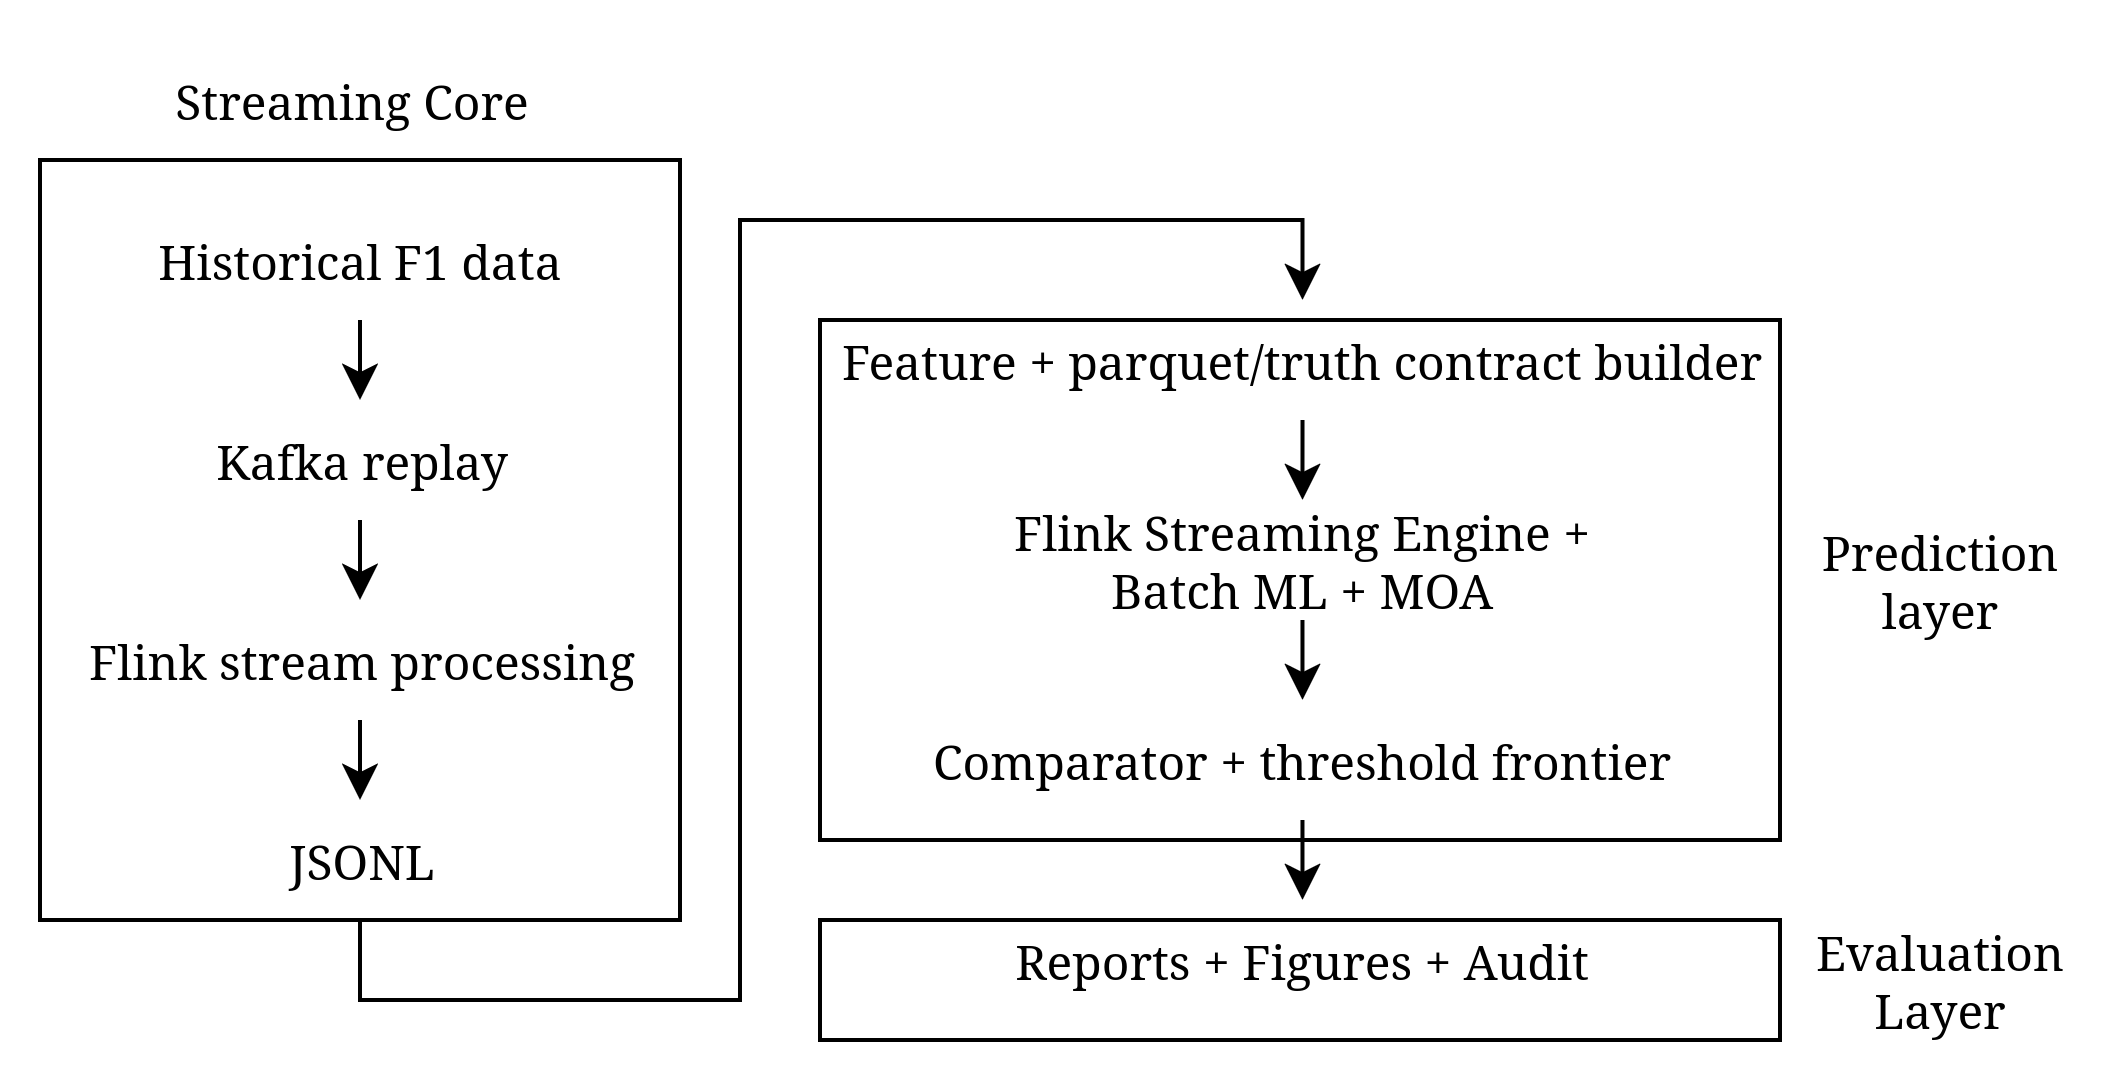
\includegraphics[width=0.75\textwidth]{Images/ch4/full_architecture.png}
    \caption{High-level architecture of the pipeline.}
    \label{fig:full_architecture}
\end{figure}


\subsection{Ingestion and Replay Architecture}

The pipeline starts in the Streaming Core Layer with the event sourcing stage. In this stage, a Python script retrieves historical race data from FastF1 and prepares the first
replayable representation of the race. The extracted data are cleaned, normalized, and enriched with the fields required by the replay and strategy pipeline. The details of
this preparation step are discussed later in Section~\ref{sec:historical_race_replay}. At this level, the relevant architectural point is that the race is prepared once and stored as a Parquet artifact,
so that the same session can be replayed multiple times without repeating the extraction process.

The replay stage is handled by a second Python script. This script reads the prepared Parquet data and publishes the race events to Kafka, race by race. The replay follows the
original event time of the race, so the order of the streamed observations reflects the natural progression of the session rather than the speed at which the experiment is executed.
This separation between preparation and replay makes the stream controllable: the same race snapshot can be replayed again for debugging, regeneration of artifacts, or comparison
between different downstream configurations.

Kafka organizes the replay into three topics with different granularities: telemetry, laps, and track status. The telemetry topic contains the highest-frequency stream and describes
continuous car-level signals. The laps topic emits one event per driver and completed lap, carrying more aggregated information such as lap time, position, tyre life, stint information,
and pit-related markers. The track-status topic is sparser and represents global race conditions, such as yellow flags, virtual safety cars, safety cars, and similar session-level
events. Keeping these streams separated allows the processing layer to combine high-frequency car behaviour, lap-level race state, and global race context when needed.

The ingestion and replay architecture therefore provides a reproducible entry point for the whole system. Historical data are fetched, prepared, stored once, and then streamed
through Kafka in a consistent and analyzable form. This supports the main experimental requirement of the pipeline: the same historical race can be replayed several times while
preserving the same input evidence for the following Flink, learning, and evaluation stages.

\begin{figure}[htbp]
    \centering
    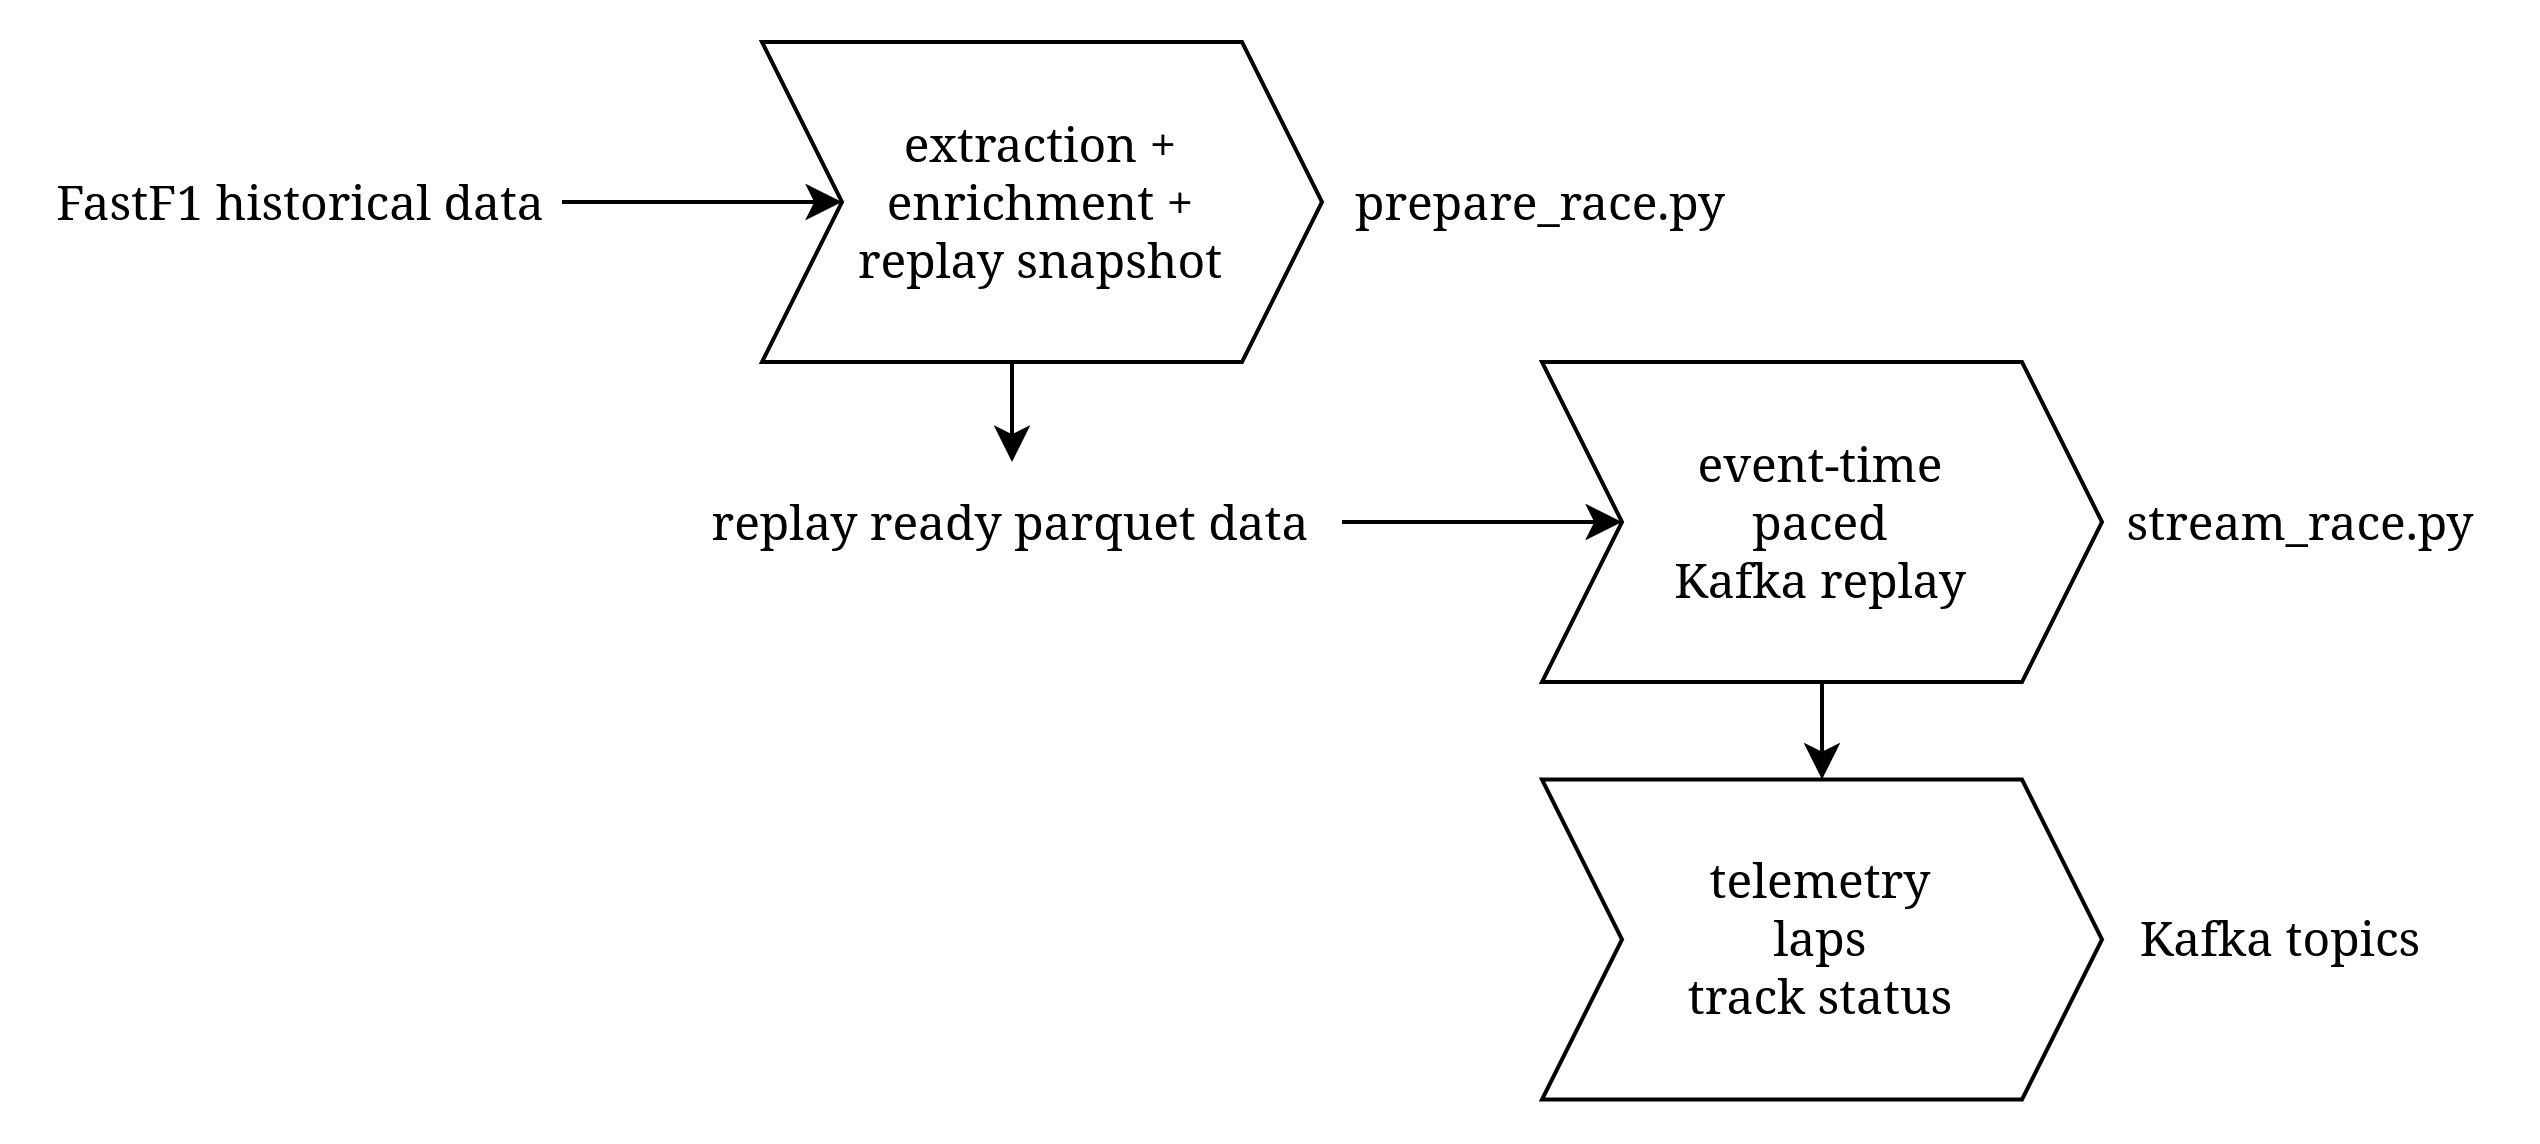
\includegraphics[width=0.75\textwidth]{Images/ch4/ingestion&replay.png}
    \caption{Ingestion and replay architecture. Historical race data are extracted and stored once as replay-ready Parquet artifacts, then replayed through Kafka as telemetry,
        lap, and track-status streams.}
    \label{fig:ingestion_replay_architecture}
\end{figure}


\subsection{Flink Stream-Processing Architecture}

After the replay stage publishes the race topics to Kafka, Flink consumes them and becomes the main stream-processing component of the system. Its role is to transform the 
incoming race streams into race-aware strategy signals and persistent artifacts. The processing follows event time, so the state of the race is updated according to the original 
race chronology rather than according to the execution speed of the replay.

At this architectural level, the relevant point is that Flink maintains the evolving race context needed by the downstream components. Event-time processing is used to order 
race observations, state is used to remember information such as track status, gaps, tyre history, and previous driver context, while windows group events around race and lap-level 
situations. On top of this stateful layer, strategy operators compute the main intermediate signals used by the system, including rival context, tyre drops, drop zones, pit evaluations, 
and pit suggestions. The detailed logic used to construct these signals is described later in Sections~\ref{sec:race_context_building} and~\ref{sec:pit_suggestion_and_classification}.

The output of this stage has two forms. Live alerts are sent back to Kafka so that they can be consumed during the replay, while JSONL artifacts are persisted to the data lake 
and reused by the feature, learning, and evaluation stages. Flink therefore acts as the boundary between live-like stream processing and reproducible downstream analysis.

\begin{figure}[htbp]
    \centering
    
\includegraphics[width=0.75\textwidth]{Images/ch4/flink.png}
    \caption{Flink stream-processing architecture. Kafka topics are consumed with event-time semantics, enriched through stateful race context, and transformed into strategy signals, live alerts, and persisted JSONL artifacts.}
    \label{fig:flink_stream_processing_architecture}
\end{figure}

\subsection{Data Lake and Feature Architecture}

After the Flink processing stage, the stream outputs are persisted in the data lake as JSONL artifacts. This storage step defines the boundary between the live-like streaming part of 
the system and the reproducible learning and evaluation part. The same race replay can generate live alerts during execution, but the downstream models and comparators require 
stable files that can be inspected, joined, and reused without running the stream again.

The data lake contains several families of artifacts. The pit timing and pit evaluation outputs describe the truth side of the problem, since they record real pit events and the 
post-pit outcome labels. The drop-zone and tyre-degradation outputs describe additional race context generated by the stream-processing logic. The pit suggestion stream stores the 
rule-based decisions emitted by the Flink Strategy Engine, while the ML feature stream stores the per-driver, per-lap rows used by the learning pipeline.

Dataset preparation starts from these JSONL files and converts them into a Parquet training dataset. This step performs deduplication, joins the different stream outputs, removes 
fields that would introduce target leakage, and builds the horizon-based labels used by the prediction contracts. The resulting dataset is therefore 
a structured representation of the same stream artifacts produced by Flink.

Dataset preparation also defines the feature contract used by the learning branches.
This step applies feature filtering and selected feature transformations, fields that would expose target information or shortcut information are removed, while some 
raw race quantities are converted into more comparable representations. For example, race progress and driver pace can be expressed as percentage features, so 
that the learner receives values that are less tied to a specific circuit length or absolute lap time scale. The detailed motivation for source-year removal and the percent 
feature profile is discussed later in Section~\ref{sec:source_year_removal} and Section~\ref{sec:percent_feature_profile}.

This architecture keeps the feature construction step traceable. The learning models do not access the original race outcome directly; they receive a filtered and aligned dataset 
derived from the persisted stream outputs. In this way, the data lake acts as the contract boundary between streaming engineering, Batch and MOA learning, and the final evaluation 
protocol.

\begin{figure}[htbp]
    \centering
    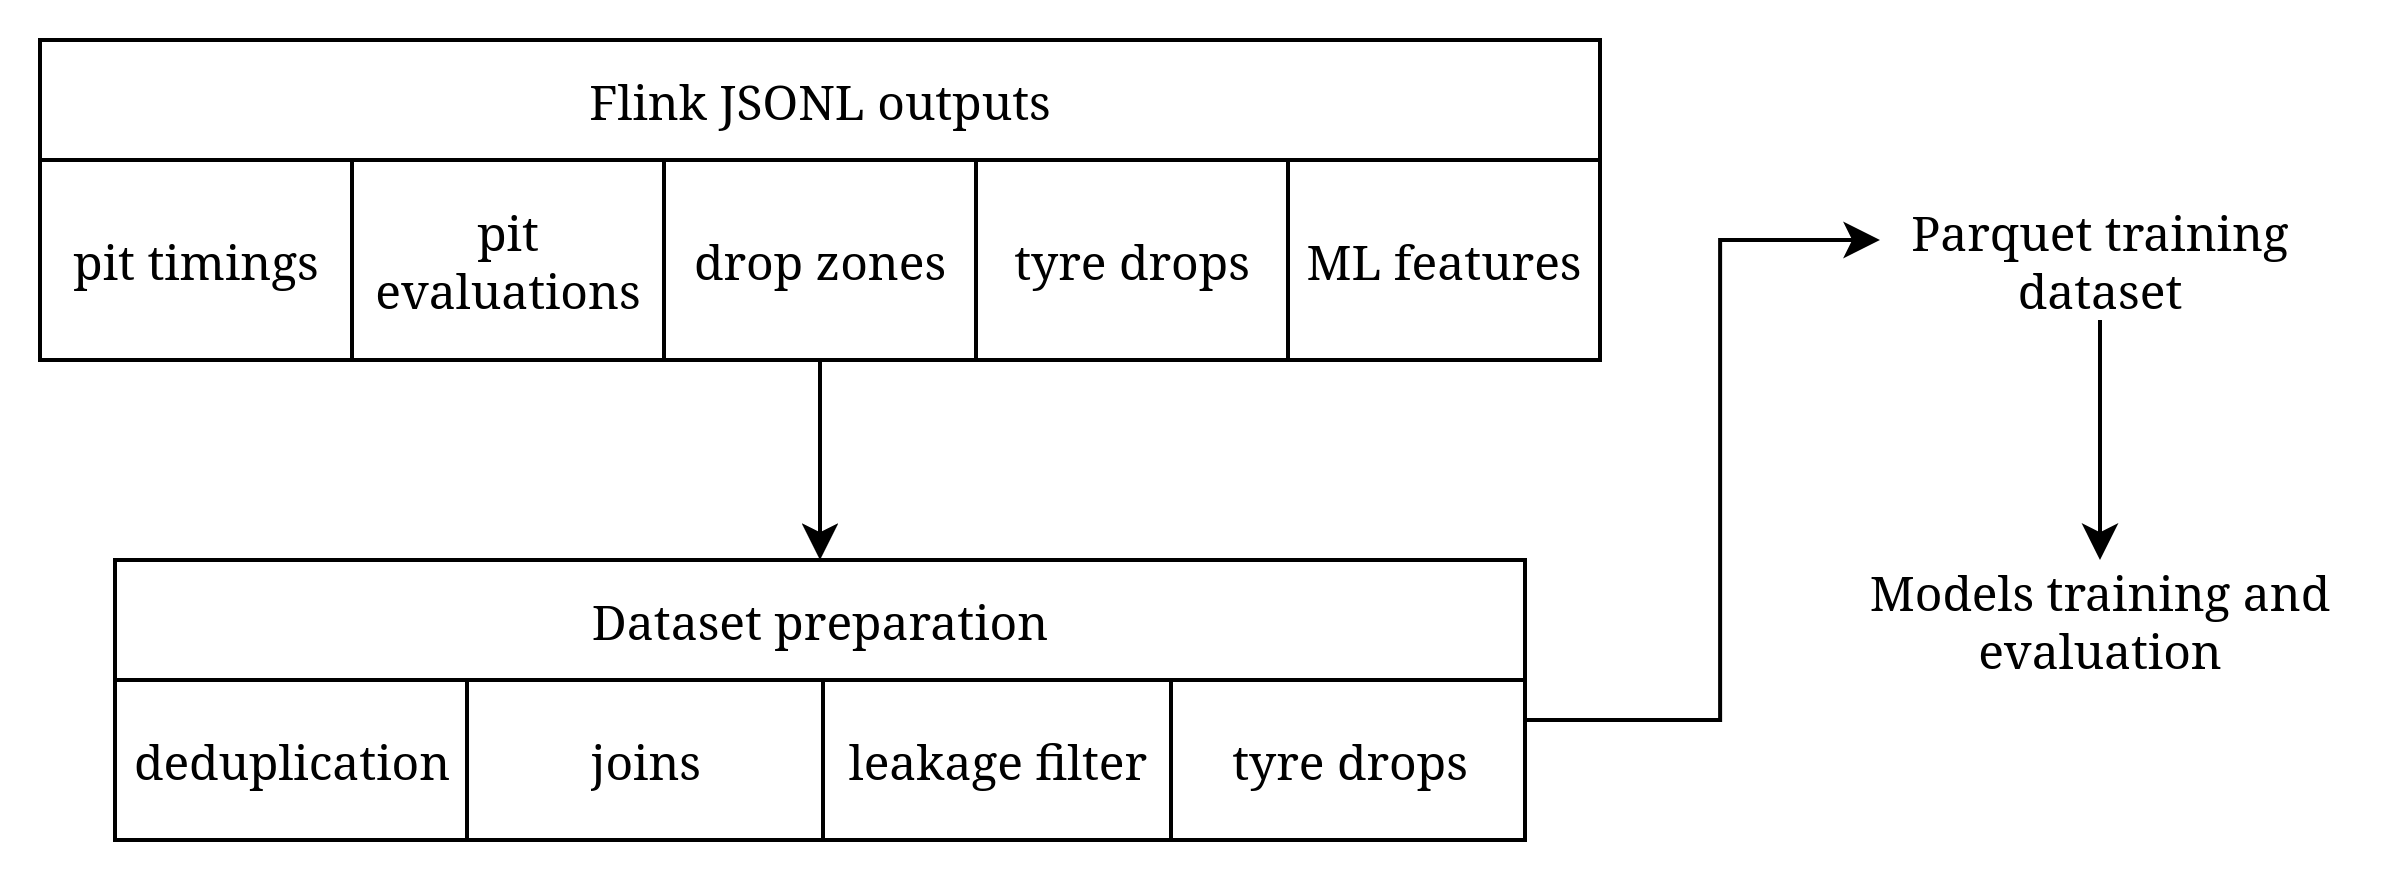
\includegraphics[width=0.75\textwidth]{Images/ch4/dataset_prep.png}
    \caption{Data lake and feature architecture.}
    \label{fig:data_lake_feature_architecture}
\end{figure}

\subsection{Truth and Comparator Architecture}

After the data lake boundary has been defined, the next architectural step is to define how predictions are compared with the truth. This layer is needed because the three decision 
systems produce different types of output. Before these outputs can be compared, they have to be converted into positive calls and matched against the same prediction contracts.

The two main contracts are \texttt{pit\_any\_h2} and \texttt{pit\_success\_h2}. In the \texttt{pit\_any\_h2} contract, a positive prediction at lap $k$ is correct if an eligible 
pit stop occurs in the following two laps, that is, in the future window $[k+1, k+2]$. This contract represents the pit timing problem. In the \texttt{pit\_success\_h2} contract, 
a positive prediction is correct only if an eligible pit stop occurs in the same window and that stop is later classified as successful by the post-pit evaluation pipeline. 
This second contract is stricter, because the system must predict both the timing of the pit and the fact that the pit will correspond to a positive strategic outcome.

The truth used for training and comparison comes from real pit events and from their classification after 
the stop has occurred. The comparator uses this truth layer to evaluate the calls produced by Flink, Batch XGBoost, and MOA with the same horizon and the same eligible event universe.


\subsection{Model Architecture}

The final architectural block concerns the way the three decision systems are connected to the common evaluation pipeline. At this point, 
the truth contracts and the feature artifacts have already been defined. The remaining issue is that the systems do not produce the same type of output, even though they 
must be evaluated under the same contracts.

The Flink Strategy Engine emits rule-based recommendation labels, such as \texttt{MONITOR}, \texttt{GOOD\_PIT}, and \texttt{PIT\_NOW}. For the operational comparison, 
\texttt{PIT\_NOW} is treated as a positive pit call. Batch XGBoost instead produces out-of-fold probability scores, while the MOA Online Learner produces vote-based 
scores during prequential evaluation. For both learning-based systems, positive calls are obtained by applying a selected threshold to the score.

The model architecture therefore hides the difference in output format behind a common decision representation. After conversion, each system produces the same logical 
object: a positive call associated with a race, a driver, and a lap. The comparator can then match these calls against the same future horizon truth contracts. 
In this way, the three systems keep their different decision mechanisms, while the final scoring remains shared.


\section{Implementation Experience}

% Maps to presentation slides 27--38.
%
% This section is more practical than the architecture section.
% It explains how the architecture was progressively turned into the thesis experiment.

\subsection{Historical Race Replay}
\label{sec:historical_race_replay}

% Slide 27.
%
% Goal:
% Describe implementation phase 1.
%
% Content to cover:
% \begin{itemize}
%     \item FastF1 loads a race session;
%     \item telemetry, laps, and track status are extracted;
%     \item events are enriched with gaps, weather, and pit-loss information;
%     \item events are ordered by event time;
%     \item the prepared race is saved as Parquet;
%     \item the saved race can then be streamed to Kafka with a replay speed and optional start lap.
% \end{itemize}
%
% Main phrase:
% freeze the race once, then replay it many times as a controlled live-like stream.

\subsection{Persisted Stream Outputs}
% Slide 28.
%
% Goal:
% Describe implementation phase 2.
%
% Content to cover:
% \begin{itemize}
%     \item Flink converts race streams into persisted strategy artifacts;
%     \item truth artifacts include \texttt{pit\_timings} and \texttt{pit\_evals};
%     \item race-context artifacts include \texttt{drop\_zones}, \texttt{tire\_drops}, and \texttt{lift\_coast};
%     \item decision-stream artifacts include \texttt{pit\_suggestions};
%     \item ML-contract artifacts include \texttt{ml\_features};
%     \item these JSONL outputs connect live stream processing to reproducible Batch/MOA evaluation.
% \end{itemize}

\subsection{Race Context Building in Flink}
\label{sec:race_context_building}
% Slide 29.
%
% Goal:
% Explain which context metrics are built in the stream.
%
% Content to cover:
% \begin{itemize}
%     \item gaps and rivals are built by ordering drivers by lap position and computing local gap context;
%     \item tyre degradation compares current lap pace against stint-best pace;
%     \item drop zone estimates where the car would rejoin if it pitted;
%     \item track status is broadcast into the strategy logic;
%     \item these metrics feed both strategy alerts and ML feature rows.
% \end{itemize}
%
% Optional formulas from slide:
% \begin{itemize}
%     \item \texttt{paceRatio = (lapTime - stintBest) / stintBest}
%     \item tyre drop condition based on \texttt{lapTime > stintBest * (1 + theta)}
%     \item drop-zone computation based on accumulated gaps and pit loss
% \end{itemize}

\subsection{Pit Suggestion and Pit Classification Logic}
\label{sec:pit_suggestion_and_classification}
% Slide 30.
%
% Goal:
% Explain why the implementation keeps two paths separate.
%
% Content to cover:
% \begin{itemize}
%     \item pit suggestion happens before the pit;
%     \item pit classification happens after a real pit;
%     \item suggestion labels include \texttt{MONITOR}, \texttt{GOOD\_PIT}, \texttt{PIT\_NOW}, and \texttt{LOST\_CHANCE};
%     \item pit classification produces success, failure, or unresolved labels;
%     \item the pit suggestion score combines pace, track status, traffic, strategy penalty, urgency, timing pressure, end-of-race penalty, competitive pressure, and uncertainty penalty;
%     \item post-pit outcome classification compares post-pit and pre-pit gap conditions.
% \end{itemize}



\subsection{Addressing Invalid Data and Leakage Risks}

% Slide 31.
%
% Goal:
% Explain the corrections that were needed to turn the working pipeline into a fair thesis experiment.
%
% Content to cover:
% \begin{itemize}
%     \item different race/event universes required a shared canonical truth universe;
%     \item past/future contamination required chronological or race-wise evaluation;
%     \item target leakage required removing target, truth, matched-pit, and eligibility fields;
%     \item ambiguous truth definitions required explicit truth lenses;
%     \item shortcut features required removing \texttt{\_source\_year}.
% \end{itemize}


\subsection{Flink Strategy Engine Variants}

% Slide 32.
%
% Goal:
% Explain implementation phase 4.
%
% Content to cover:
% \begin{itemize}
%     \item the rule-based baseline was tuned before the final Batch/MOA comparison;
%     \item the Strict version was conservative and disabled promotion mechanisms;
%     \item the Rival-pressure version increased reach by enabling rival-pressure promotion;
%     \item the Guarded rival-pressure version kept rival pressure but added guards against noisy promotions;
%     \item the guarded version was frozen as the final Flink Strategy Engine version.
% \end{itemize}


\subsection{Batch ML Pipeline}

% Slide 33.
%
% Goal:
% Explain implementation phase 5.
%
% Content to cover:
% \begin{itemize}
%     \item Batch ML is expressed as race-sequential out-of-fold evaluation;
%     \item for each held-out race, training uses previous races;
%     \item XGBoost predicts scores on the held-out race;
%     \item out-of-fold scores are appended into a table;
%     \item thresholds are swept on OOF scores;
%     \item feature filtering removes metadata, target fields, truth fields, and matched-pit fields;
%     \item XGBoost is used as a binary logistic classifier with \texttt{aucpr};
%     \item calibration is treated as probability-quality diagnostic, not as a guarantee.
% \end{itemize}


\subsection{Source-Year Removal}
\label{sec:source_year_removal}
% Slide 34.
%
% Goal:
% Explain implementation phase 6.
%
% Content to cover:
% \begin{itemize}
%     \item the first dataset contained \texttt{source\_year};
%     \item \texttt{source\_year} could encode season-level shortcuts;
%     \item SHAP exposed it as an important feature;
%     \item after removal, feature importance shifted toward race-state features such as tyre life, race progress, and pace signals.
% \end{itemize}


\subsection{Percent Feature Profile}
\label{sec:percent_feature_profile}
% Slide 35.
%
% Goal:
% Explain implementation phase 7.
%
% Content to cover:
% \begin{itemize}
%     \item some raw race values were transformed into race-relative signals;
%     \item \texttt{race\_progress\_pct} describes where the car is in the race;
%     \item \texttt{lapTime\_vs\_driver\_prev\_mean\_pct} describes current pace relative to previous driver pace;
%     \item conservative exclusions remove team and rainfall from this profile;
%     \item Percent is an engineered profile partly motivated by Batch explainability;
%     \item No-Year remains the cleaner neutral baseline;
%     \item the same feature contract is exported to both Batch and MOA.
% \end{itemize}


\subsection{MOA Export}

% Slide 36.
%
% Goal:
% Explain implementation phase 8.
%
% Content to cover:
% \begin{itemize}
%     \item MOA requires a different input format from XGBoost;
%     \item the export step converts the Batch feature matrix into a MOA-compatible stream dataset;
%     \item the matrix contract is preserved;
%     \item exported elements include CSV, ARFF, schema JSON, and binary target labels;
%     \item Batch and MOA differ in learning paradigm, not in input semantics.
% \end{itemize}


\subsection{MOA Prequential Evaluation}

% Slide 37.
%
% Goal:
% Explain implementation phase 9.
%
% Content to cover:
% \begin{itemize}
%     \item streaming ML is evaluated in stream order;
%     \item for each instance, the learner predicts first;
%     \item the prediction and vote information are logged;
%     \item the learner then trains on the same instance;
%     \item this preserves the test-then-train order;
%     \item the current prediction cannot use future rows.
% \end{itemize}


\subsection{MOA Vote Logger}

% Slide 38.
%
% Goal:
% Explain implementation phase 10.
%
% Content to cover:
% \begin{itemize}
%     \item initial MOA output was mostly hard 0/1 labels;
%     \item hard labels made threshold sweeps weak;
%     \item the custom logger records class votes before training on the instance;
%     \item \texttt{positive\_score = vote\_1 / (vote\_0 + vote\_1)};
%     \item the learning protocol remains unchanged;
%     \item continuous vote scores enable AP, PR curves, and threshold-frontier diagnostics.
% \end{itemize}


\section{Chapter Summary}

% Briefly close the chapter:
% the architecture creates a reproducible path from historical races to stream artifacts,
% and the implementation experience shows how the Flink, Batch, and MOA branches were made
% comparable under the same contracts.
% The quantitative comparison is left to Chapter~\ref{ch:experimental_evaluation}.
\chapter{Experimental Evaluation}
\label{ch:experimental_evaluation}

This chapter evaluates the resulting systems under a fixed experimental protocol,
the goal is to compare the behaviour of the Flink Strategy Engine, Batch XGBoost, and the MOA Online Learner on the same pit decision contracts.

The evaluation is organized around the two targets introduced earlier: \texttt{pit\_any\_h2}, which measures whether a pit stop is predicted within the evaluation
horizon, and \texttt{pit\_success\_h2}, which measures whether a successful evaluated pit stop is predicted. The chapter first defines the frozen protocol, then reports
the rule engine baseline, the training and runtime characteristics of the learning branches, the headline comparison for pit timing, and the stricter comparison for successful
pit calls.
% The final part discusses diagnostic views that help interpret the differences between operational precision, event coverage, and matched-pit success rate.

\section{Evaluation Scope and Frozen Protocol}

Before presenting the results, the evaluation protocol is fixed explicitly. This is necessary because the systems do not produce the same type of output and do not naturally
operate on identical tables as described in Chapter \ref{ch:problem_solving} Section \ref{sec:corrections}. The Flink Strategy Engine emits rule based recommendation labels,
Batch XGBoost emits out-of-fold probability scores, and MOA emits vote based scores
in prequential order. The protocol defines how these outputs are converted into comparable positive calls and how those calls are matched against truth.
All headline results are computed on seasons 2022--2025, which is the ground effect F1 car era. The truth universe mode is \texttt{canonical\_sde\_truth}, and the main lens is \texttt{clean\_actionable}. This means
that the comparison uses the shared SDE-defined truth universe and removes cases that are not considered fair actionable strategy decisions under the clean lens. By doing so
comparing systems on different race, driver, or event populations is avoided.

Two targets are evaluated. The first target, \texttt{pit\_any\_h2}, measures pit timing: a positive call is correct when an eligible pit stop is matched within the timing
contract. The second target, \texttt{pit\_success\_h2}, measures successful pit-call prediction: a positive call is correct only when an eligible future pit stop is matched
and the post pit evaluator classifies that stop as successful. For this second contract, failed or disadvantage pit outcomes are treated as negatives, while unresolved,
weather related, and unmapped outcomes are excluded from the clean success truth.
Both are described at \ref{ch:problem_framing} Section \ref{sec:contracts}.

The compared systems are:
\begin{itemize}
    \item the frozen Flink Strategy Engine profile
    \item Batch XGBoost with the No-Year feature profile
    \item Batch XGBoost with the Percent feature profile
    \item MOA Online Learner with the No-Year feature profile
    \item MOA Online Learner with the Percent feature profile
\end{itemize}

The Batch systems are evaluated with race sequential out-of-fold predictions. Each score is produced on a race that was not used in the corresponding training prefix.
The MOA systems are evaluated with the prequential test-then-train protocol where each row is predicted first and then used for learning. The Flink Strategy Engine is evaluated
from its persisted \texttt{pit\_suggestions} artifacts, with the selected frozen rule profile.

The evaluation artifacts were also checked for protocol consistency before reporting the results. In particular, the \texttt{pit\_success\_h2} evaluation uses the corrected success
contract: a positive call is matched only against future pit evidence, positive calls from the system without a real match are counted as false positives,
and matched-pit success rate is kept only as a diagnostic measure.
This distinction is important because successful pit call prediction is stricter than pit timing,
counting these no match calls as false positives gives a more realistic operational view of the system behaviour.



\section{Flink Strategy Engine Baseline and Freeze Decision}

As described in Section~\ref{sec:flink_tuning}, the Flink Strategy Engine was not used in its first rule configuration. Several deterministic variants were tested before
comparing the rule based system with Batch XGBoost and MOA. This step was needed to obtain a stable rule baseline, while keeping the later comparison independent from the
tuning of the learning models.

The first variant was the strict profile. In this configuration, the engine mainly relied on the base score, timing gates, and actionability gates. Optional promotion
mechanisms were disabled, especially the rival pressure promotion. This made the system conservative: it emitted fewer strong pit calls and avoided some noisy recommendations,
but it also missed situations where nearby rivals created a relevant strategic pressure.

The second variant enabled rival pressure. In this configuration, recent pit activity from nearby rivals could promote a near actionable situation into a stronger
recommendation. The objective was to increase the reach of the Flink Strategy Engine, especially in cases where waiting could lose a strategic window. This improved recall, but
it also introduced more noisy calls.

The final variant kept the rival pressure mechanism but added guards. Promotions were allowed only when the surrounding context supported the call, for example through
timing pressure, urgency, recent lap constraints, and gap conditions. This guarded profile was selected as the frozen Flink Strategy Engine baseline. After this point, the
rule engine configuration was kept fixed and the Batch and MOA systems were compared against it under the same evaluation protocol.

Table~\ref{tab:flink_strategy_engine_freeze} summarizes the tuning trajectory. The strict profile is the most conservative one. The rival pressure profile increases reach,
but loses precision. The frozen guarded profile recovers precision while keeping the same $F_{0.5}$ value as the rival pressure configuration.

\begin{table}[htbp]
    \centering
    \caption{Flink Strategy Engine variant comparison before freezing the deterministic baseline.}
    \label{tab:flink_strategy_engine_freeze}
    \begin{tabular}{lcccl}
        \toprule
        Variant               & Precision & Recall & $F_{0.5}$ & Interpretation                       \\
        \midrule
        Strict                & 0.232     & 0.068  & 0.156     & Stable but conservative              \\
        Rival pressure        & 0.218     & 0.097  & 0.174     & Better reach, more noise             \\
        Flink Strategy Engine & 0.248     & 0.079  & 0.174     & Recovered precision, equal $F_{0.5}$ \\
        \bottomrule
    \end{tabular}
\end{table}

The selected profile is the deterministic baseline obtained from the rule engine tuning stage.
The following sections use this frozen Flink Strategy Engine when comparing the three decision paradigms.

\begin{figure}[htbp]
    \centering
    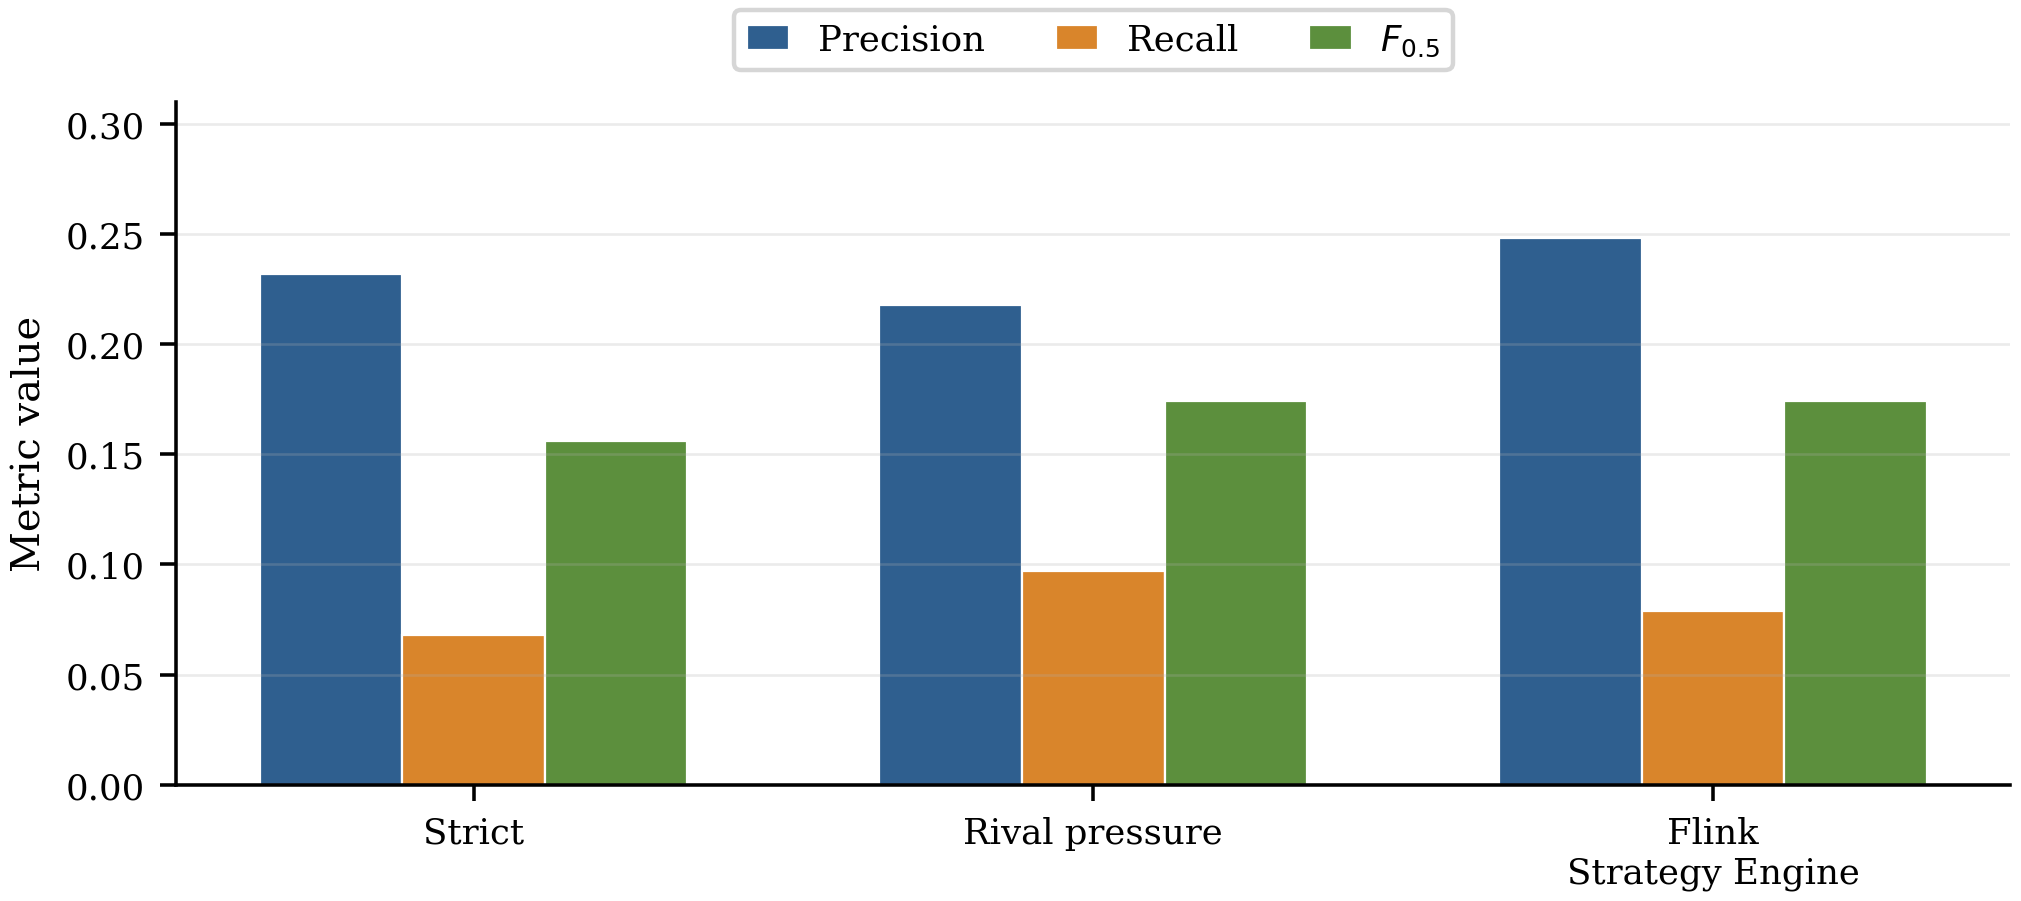
\includegraphics[width=0.98\textwidth]{Images/ch5/rule_engine_tuning_variants_clean.png}
    \caption{Rule-engine tuning summary for 2025 under the clean\_actionable lens, showing pit\_any\_h2 precision, recall, and $F_{0.5}$ across the three rule-engine variants.}
    \label{fig:rule_engine_tuning_variants_clean}
\end{figure}

\section{Training Runtime Comparison}

The first experimental comparison concerns the runtime of the two learning branches. The values in Table~\ref{tab:training_runtime_comparison} report the learner runtime for
each profile and target. Dataset preparation and MOA export are treated as separate stages and are not included in these times.

The difference between Batch and MOA is expected from the evaluation protocols described in Chapter~\ref{ch:problem_solving}. Batch XGBoost uses race-sequential out-of-fold
evaluation: the model is trained on the previous races, tested on the next held-out race, then trained again on a larger prefix and tested on the following race. This repeated
fitting makes the Batch branch slower. MOA instead runs once over the exported stream in prequential order. Each instance is predicted and then used for training, so
the learner processes the stream in a single pass.

\begin{table}[htbp]
    \centering
    \caption{Training and evaluation runtime by learner, feature profile, and target.}
    \label{tab:training_runtime_comparison}
    \begin{tabular}{lll}
        \toprule
        System        & Target                    & Runtime \\
        \midrule
        Batch No-Year & \texttt{pit\_any\_h2}     & 1m 44s  \\
        Batch No-Year & \texttt{pit\_success\_h2} & 1m 41s  \\
        Batch Percent & \texttt{pit\_any\_h2}     & 1m 38s  \\
        Batch Percent & \texttt{pit\_success\_h2} & 1m 29s  \\
        MOA No-Year   & \texttt{pit\_any\_h2}     & 24s     \\
        MOA No-Year   & \texttt{pit\_success\_h2} & 20s     \\
        MOA Percent   & \texttt{pit\_any\_h2}     & 18s     \\
        MOA Percent   & \texttt{pit\_success\_h2} & 13s     \\
        \bottomrule
    \end{tabular}
\end{table}

The timing results should therefore be interpreted as runtime evidence for the selected evaluation implementation, not as a general benchmark of
XGBoost against MOA. In this pipeline, MOA is faster mainly because it uses a single prequential pass, while Batch XGBoost repeatedly fits models across
race-sequential folds.


\section{Pit Timing Headline Results (\texttt{pit\_any\_h2})}

The first headline comparison concerns the \texttt{pit\_any\_h2} contract. This target evaluates pit timing: when a system emits a positive call at a
given driver lap, the comparator checks whether an eligible pit stop occurs within the evaluation horizon. Unlike \texttt{pit\_success\_h2}, this contract does
not require the pit stop to be classified as strategically successful after the fact. It is therefore the cleaner task for measuring whether the systems can
recognize when a pit window is approaching.

The task is still strongly imbalanced. At learner-matrix level, the \texttt{clean\_actionable} \texttt{pit\_any\_h2} target contains 93,623 driver-lap rows,
but only 5,855 of them are positive rows. This means that positive pit-timing situations represent about 6.3\% of the learner rows. A low absolute precision is
therefore expected: most driver-lap situations are not close to a pit stop, so emitting a positive call is difficult and false positives are easy to produce.

The 5,855 positive rows should not be read as 5,855 distinct pit stops. They are positive driver-lap examples produced by the horizon label. Intuitively, one
real pit can make more than one previous lap positive. For example, if a driver pits on lap $k$, then the rows for laps $k-1$ and $k-2$ can both be labelled as
positive because both are close enough to the same future pit. With a two-lap horizon, each pit can therefore generate up to two positive training rows.

For event-level interpretation, the shared comparator universe contains 3,048 unique eligible pit events. This is the denominator used when discussing event
recall. The ratio between row positives and unique pit events is about $5,855/3,048=1.92$, close to but not exactly $2.00$. This is expected. Some pits occur
too early to have two valid previous rows, some horizons can overlap, and the row-level learner matrix and the shared comparator event universe are not exactly
the same object. The important point is that the two counts answer different questions: 5,855 describes how many driver-lap rows are positive for learning, while
3,048 describes how many unique pit events can be covered in the event-level comparison.

This distinction is used throughout the interpretation. Precision is computed from emitted positive calls: when the system says that a pit is coming, how often is
that call correct? Event recall measures coverage over unique eligible pit events: how many real pit events were covered by at least one valid call? The row-level
imbalance explains why high absolute precision is difficult, while the event-level denominator explains the coverage side of the evaluation.

\subsection{Interpretation Table}

Table~\ref{tab:pit_any_interpretation} reports the selected operating points for \texttt{pit\_any\_h2}.

The results show that \texttt{pit\_any\_h2} is a learnable timing task. The Flink Strategy Engine reaches good precision for a deterministic rule baseline, but its event
recall is low, which means that it covers only a limited fraction of eligible pit events. Batch No-Year improves recall over the Flink baseline, while Batch Percent
improves it further, showing that the engineered relative representation is more effective for this timing task. MOA gives the strongest precision-weighted trade-off:
both MOA profiles reach the highest $F_{0.5}$ values, with MOA No-Year slightly ahead of MOA Percent, which is understandable since the Percent features set is engineered from
Batch SHAP analysis explain later in section \ref{sec:explainability}.

\begin{table}[htbp]
    \centering
    \caption{Selected \texttt{pit\_any\_h2} operating points.}
    \label{tab:pit_any_interpretation}
    \begin{tabular}{lccc}
        \toprule
        System                & Precision & Event recall & $F_{0.5}$ \\
        \midrule
        Flink Strategy Engine & 0.271     & 0.071        & 0.173     \\
        Batch No-Year         & 0.204     & 0.122        & 0.180     \\
        Batch Percent         & 0.242     & 0.220        & 0.237     \\
        MOA No-Year           & 0.350     & 0.183        & 0.296     \\
        MOA Percent           & 0.344     & 0.182        & 0.292     \\
        \bottomrule
    \end{tabular}
\end{table}

Overall, the timing task favours the learning-based systems. Batch Percent gives the largest event coverage among the reported systems, while MOA provides the
best precision-oriented balance. This suggests that, for predicting whether a pit will happen soon, the learned models capture useful timing patterns beyond the
deterministic rule logic.

The precision values should be read in the context of the imbalance described above. Since positive pit-timing rows are a small minority of the learner matrix,
precisions in the 0.20--0.35 range are substantially above the row-level positive-rate baseline of about 0.063. At the same time, precision alone is not sufficient:
a system can be precise but cover few real pit events. This is why the table reports precision together with event recall and $F_{0.5}$.


\subsection{Headline Figure}

Figure~\ref{fig:pit_any_headline_comparison} shows the same \texttt{pit\_any\_h2} comparison visually. The figure makes the trade-off between precision,
event recall, and $F_{0.5}$ easier to inspect across the deterministic Flink Strategy Engine and the learning-based systems.

\begin{figure}[htbp]
    \centering
    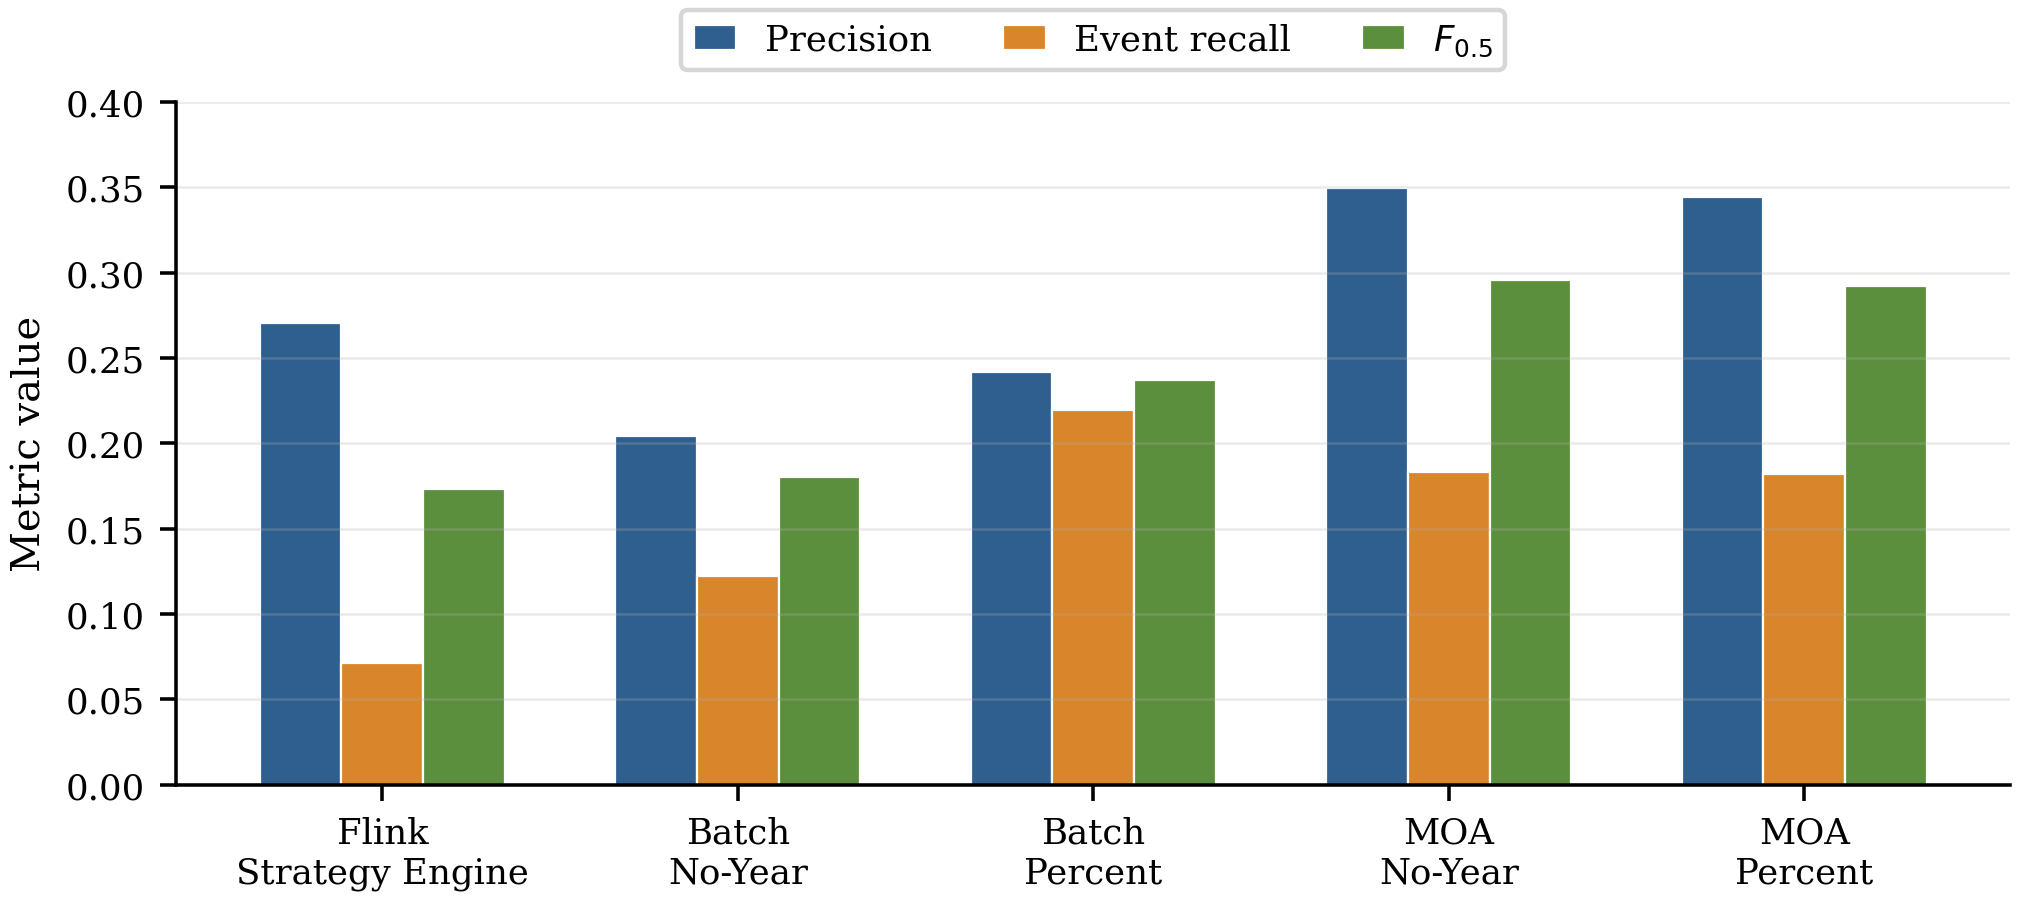
\includegraphics[width=0.99\textwidth]{Images/ch5/pit_any_headline_comparison.png}
    \caption{\texttt{pit\_any\_h2} headline comparison under the \texttt{canonical\_sde\_truth} universe and \texttt{clean\_actionable} lens. The figure
        reports precision, event recall, and $F_{0.5}$ for the selected operating points of the compared systems.}
    \label{fig:pit_any_headline_comparison}
\end{figure}

The visual comparison confirms the same interpretation as Table~\ref{tab:pit_any_interpretation}: learned models improve the timing task over the
deterministic rule baseline, with Batch Percent giving the largest event recall and MOA giving the strongest precision-oriented balance.


\section{Accounting Semantics and \texttt{pit\_success\_h2} Strict Contract}

Before presenting the \texttt{pit\_success\_h2} results, the accounting semantics must be clarified. The success contract is stricter than the pit timing contract because a
positive call is correct only if an eligible future pit happens and that pit is later classified as successful.

This creates a distinction between decision-level quantities and event-level quantities. A system emits positive calls at driver-lap level, while the truth is defined by
pit events and post-pit outcome labels. For this reason, the metrics used in this section do not all have the same denominator. The evaluation separates three quantities:
strict precision, successful event coverage, and matched-pit success rate.

\subsection{Decision-vs-Event Ledger Clarification}

The first quantity is strict precision. This is the main operational precision used for the \texttt{pit\_success\_h2} comparison. A positive call is counted as a true
positive only if it matches an eligible future pit whose outcome is successful. A positive call with no matched pit is counted as a false positive, because the system
still emitted a successful-pit recommendation that did not correspond to an eligible future pit. A positive call matched to a failed or disadvantage pit is also counted
as a false positive. In compact form:

\[
    strictPrecision =
    \frac{TP}{TP + FP_{no\_match} + FP_{failure}}.
\]

The second quantity is successful event coverage, which is an event-level measure. It counts how many eligible successful pit events were covered by at least one positive call.
Its denominator is the number of eligible successful pit events in the truth universe:

\[
    successfulEventCoverage =
    \frac{coveredSuccessfulEvents}{eligibleSuccessfulEvents}.
\]

This quantity is useful because a system can have reasonable precision while still missing most successful pit opportunities.

The third quantity is matched-pit success rate. This is a diagnostic measure only. It considers only the positive calls that matched a known pit event, and then checks how
many of those matched pits were successful:

\[
    matchedPitSuccessRate =
    \frac{matchedSuccess}{matchedSuccess + matchedFailure}.
\]

This value is not the same as operational precision because it ignores positive calls that did not match any eligible pit. It therefore describes the quality of calls after
a pit match has already occurred, but it does not describe the full operational behaviour of the system. For this reason, matched-pit success rate is not used as the main
precision metric in the headline comparison.

The following sections use strict precision and successful event coverage for the main \texttt{pit\_success\_h2} comparison. Matched-pit success rate is kept separate as
a diagnostic quantity.

\subsection{Strict \texttt{pit\_success\_h2} Table and Sensitivity}

Table~\ref{tab:pit_success_selected} reports the selected strict \texttt{pit\_success\_h2} operating points for all compared systems. For the Flink Strategy Engine,
the positive call is the deterministic \texttt{PIT\_NOW} label. For Batch XGBoost and MOA, the positive call is obtained by applying the selected threshold to the model score.

The selected results confirm that \texttt{pit\_success\_h2} is substantially harder than \texttt{pit\_any\_h2}, the Flink Strategy Engine covers more successful events
than the selected learning policies, but it does so by emitting many more positive calls. Once no-match calls and failed matched pits are counted as false positives,
its strict precision is low. The selected learning policies are more conservative: they emit fewer calls, obtain higher strict precision, but cover only a small fraction
of successful pit events.

Among the selected learning policies, MOA Percent obtains the highest strict precision and the best $F_{0.5}$ score. MOA No-Year follows with lower coverage and lower
precision, while the two Batch configurations remain more conservative in terms of emitted calls and successful event coverage.

\begin{table}[htbp]
    \centering
    \caption{Selected strict \texttt{pit\_success\_h2} operating points.}
    \label{tab:pit_success_selected}
    \begin{tabular}{lccccc}
        \toprule
        System                & \shortstack{Threshold                                \\Rule} & Predicted + & \shortstack{Strict\\precision} & \shortstack{Success\\coverage} & $F_{0.5}$ \\
        \midrule
        Flink Strategy Engine & \texttt{PIT\_NOW}     & 1235 & 0.080 & 0.083 & 0.081 \\
        Batch No-Year         & 0.37                  & 46   & 0.239 & 0.010 & 0.044 \\
        Batch Percent         & 0.51                  & 51   & 0.196 & 0.009 & 0.040 \\
        MOA No-Year           & 0.58                  & 52   & 0.288 & 0.014 & 0.059 \\
        MOA Percent           & 0.58                  & 86   & 0.365 & 0.029 & 0.111 \\
        \bottomrule
    \end{tabular}
\end{table}

The selected points are intentionally strict, they show the behaviour of each system under the frozen operating policy. However, the threshold frontier also makes it
possible to inspect how the learned systems behave when the threshold is relaxed. Table~\ref{tab:pit_success_relaxed} reports this sensitivity check for the Percent profiles.

The relaxed rows are diagnostic only since they are not the main headline policy. Their purpose is to show the trade-off between call volume, strict precision, and successful
event coverage. Lowering the threshold increases the number of emitted calls and covers more successful pit events, but it also accepts more false positives. Batch
Percent increases from 51 to 844 positive calls and from $0.009$ to $0.083$ coverage, while precision drops from $0.196$ to $0.105$. MOA Percent increases from 86 to
900 positive calls and from $0.029$ to $0.169$ coverage, while precision drops from $0.365$ to $0.205$.

\begin{table}[htbp]
    \centering
    \caption{Relaxed diagnostic sensitivity points for \texttt{pit\_success\_h2} Percent profiles.}
    \label{tab:pit_success_relaxed}
    \begin{tabular}{lccccc}
        \toprule
        System                & Threshold & Predicted + & \shortstack{Strict                 \\precision} & \shortstack{Success\\coverage} & $F_{0.5}$ \\
        \midrule
        Batch Percent relaxed & 0.22      & 844         & 0.105              & 0.083 & 0.100 \\
        MOA Percent relaxed   & 0.51      & 900         & 0.205              & 0.169 & 0.196 \\
        \bottomrule
    \end{tabular}
\end{table}

Figure~\ref{fig:pit_success_apples_to_apples_main} visualizes the selected strict comparison. The figure highlights the main result of this subsection: \texttt{pit\_success\_h2}
is both rarer and stricter than pit timing, because positive calls are penalized when they do not match an eligible future pit or when the matched pit is not successful.

\begin{figure}[htbp]
    \centering
    
\includegraphics[width=0.95\textwidth]{Images/ch5/pit_success_apples_to_apples_main.png}
    \caption{Strict \texttt{pit\_success\_h2} comparison under the \texttt{canonical\_sde\_truth} universe and \texttt{clean\_actionable} lens. The figure reports strict precision,
        successful event coverage, and $F_{0.5}$ for the selected operating points.}
    \label{fig:pit_success_apples_to_apples_main}
\end{figure}





\section{Flink Strategy Engine: Diagnostic Quality vs Operational Precision}

The Flink Strategy Engine also requires a separate diagnostic view. Its \texttt{PIT\_NOW} calls often match pit stops that are later classified as successful,
but this does not mean that the engine has high operational precision under the strict \texttt{pit\_success\_h2} contract.

The reason is the denominator, matched-pit success rate only considers calls that matched a known pit event. It ignores calls that did not match any eligible future pit.
Strict precision, instead, includes those no-match calls as false positives. Therefore, matched-pit success rate can be high while strict operational precision remains low.

For \texttt{PIT\_NOW}, the matched-pit success rate is $0.583$, while strict precision is $0.080$. When \texttt{GOOD\_PIT} is added to the positive-call definition, the
matched-pit success rate increases to $0.628$, but strict precision decreases to $0.060$. This means that, conditional on matching a pit, many Flink calls correspond to
successful outcomes. However, the engine also emits many calls that do not match an eligible future pit, and those calls reduce operational precision.

\begin{table}[htbp]
    \centering
    \caption{Flink Strategy Engine diagnostic quality versus strict operational precision.}
    \label{tab:sde_diagnostic_vs_operational}
    \begin{tabular}{lcc}
        \toprule
        Positive-call definition               & Matched-pit success rate & Strict precision \\
        \midrule
        \texttt{PIT\_NOW}                      & 0.583                    & 0.080            \\
        \texttt{PIT\_NOW} + \texttt{GOOD\_PIT} & 0.628                    & 0.060            \\
        \bottomrule
    \end{tabular}
\end{table}

Figure~\ref{fig:sde_diagnostic_operational_vs_matched} visualizes the same distinction. The matched-pit success rate is useful for understanding the quality of calls after
a pit match has occurred.

\begin{figure}[htbp]
    \centering
    
\includegraphics[width=0.85\textwidth]{Images/ch5/pit_success_sde_diagnostic_operational_vs_matched.png}
    \caption{Flink Strategy Engine diagnostic matched-pit success rate compared with strict operational precision. Matched-pit success rate is diagnostic only and is not
        the headline precision metric.}
    \label{fig:sde_diagnostic_operational_vs_matched}
\end{figure}


\section{Cross-Task Headline Synthesis}

The two headline tasks show different behaviours, the \texttt{pit\_any\_h2} contract is the cleaner timing task. It only asks whether a pit stop happens soon,
so the systems are evaluated on their ability to recognize an approaching pit window. Under this contract, the learning-based systems improve over the deterministic
Flink Strategy Engine. Batch Percent gives the largest event recall, while MOA provides the strongest precision-oriented balance.

The \texttt{pit\_success\_h2} contract is stricter, a correct positive call must match a future eligible pit and that pit must be classified as successful.
This makes the task sparser and more sensitive to the threshold policy. Under the selected strict operating points, MOA Percent gives the cleanest successful-pit
calls, with the highest strict precision and the best $F_{0.5}$ among the selected learning policies. However, its successful event coverage remains low, which
shows that the task is still difficult even for the best selected learner.

The Flink Strategy Engine plays a different role in the comparison because it remains the interpretable deterministic baseline and emits more calls than the selected
learned policies in the success task. This gives it some successful event coverage, but strict precision is low once no-match calls and failed matched pits are
counted as false positives. At the same time, its matched-pit success rate is useful diagnostically: when a Flink call does match a known pit, many of those
matched pits are successful.

Overall, the results suggest that pit timing is more learnable from the available race context than successful pit-call prediction. The learning branches are
better at ranking and thresholding pit timing situations, while the success contract exposes the harder part of the problem: distinguishing not only when a pit
will happen, but whether that future pit will also be strategically favourable under the post-pit evaluation logic.

\section{PR Curves and Average Precision (Ranking Diagnostics)}

The headline tables report selected operating points, they show what happens after each score-based system has been converted into positive calls through a threshold.
Precision-recall curves provide a complementary view: they inspect how the score behaves across many possible thresholds, before committing to one operating point.

This section therefore treats PR curves and Average Precision as ranking diagnostics. They are useful for understanding whether a model assigns higher scores to positive
rows than to negative rows, and whether a different threshold could expose a better precision-recall trade-off.

\subsection{Diagnostic framing}

Precision-recall curves are computed at row level for score based systems, Batch XGBoost produces probability scores, while MOA produces vote-based scores through the
custom logger described in Chapter~\ref{ch:problem_solving}. By sweeping a threshold over these scores, each system produces a curve showing how precision and recall
change as the positive-call policy becomes more or less aggressive.

Average Precision summarizes this row-level ranking behaviour into a single value. A higher AP means that positive rows tend to receive higher scores than negative rows.
However, AP is not the same as strict operational precision. In particular, for \texttt{pit\_success\_h2}, the headline comparison must still count no-match calls and
failed matched pits as false positives.

The Flink Strategy Engine is different. It does not produce a continuous learned score used for threshold sweeping in the same way as Batch and MOA. It emits deterministic
labels such as \texttt{MONITOR}, \texttt{GOOD\_PIT}, and \texttt{PIT\_NOW}. Therefore, in the PR figures the Flink Strategy Engine is best interpreted as a fixed operating
point rather than as a learned score curve.

The purpose of this section is to inspect whether the learned systems rank the rows in a useful way. The final comparison remains based on the selected thresholds and on
the strict accounting rules defined earlier.


\subsection{PR Figures and AP Table}

Figures~\ref{fig:pr_curve_pit_any_final} and~\ref{fig:pr_curve_pit_success_final} show the precision--recall curves for the two targets,
these plots compare the score-based systems across thresholds, so they are useful for inspecting ranking behaviour before selecting an operating point. The 
Flink Strategy Engine is shown as a fixed operating point, since it emits deterministic labels rather than a continuous learned score curve.

\begin{figure}[htbp]
    \centering
    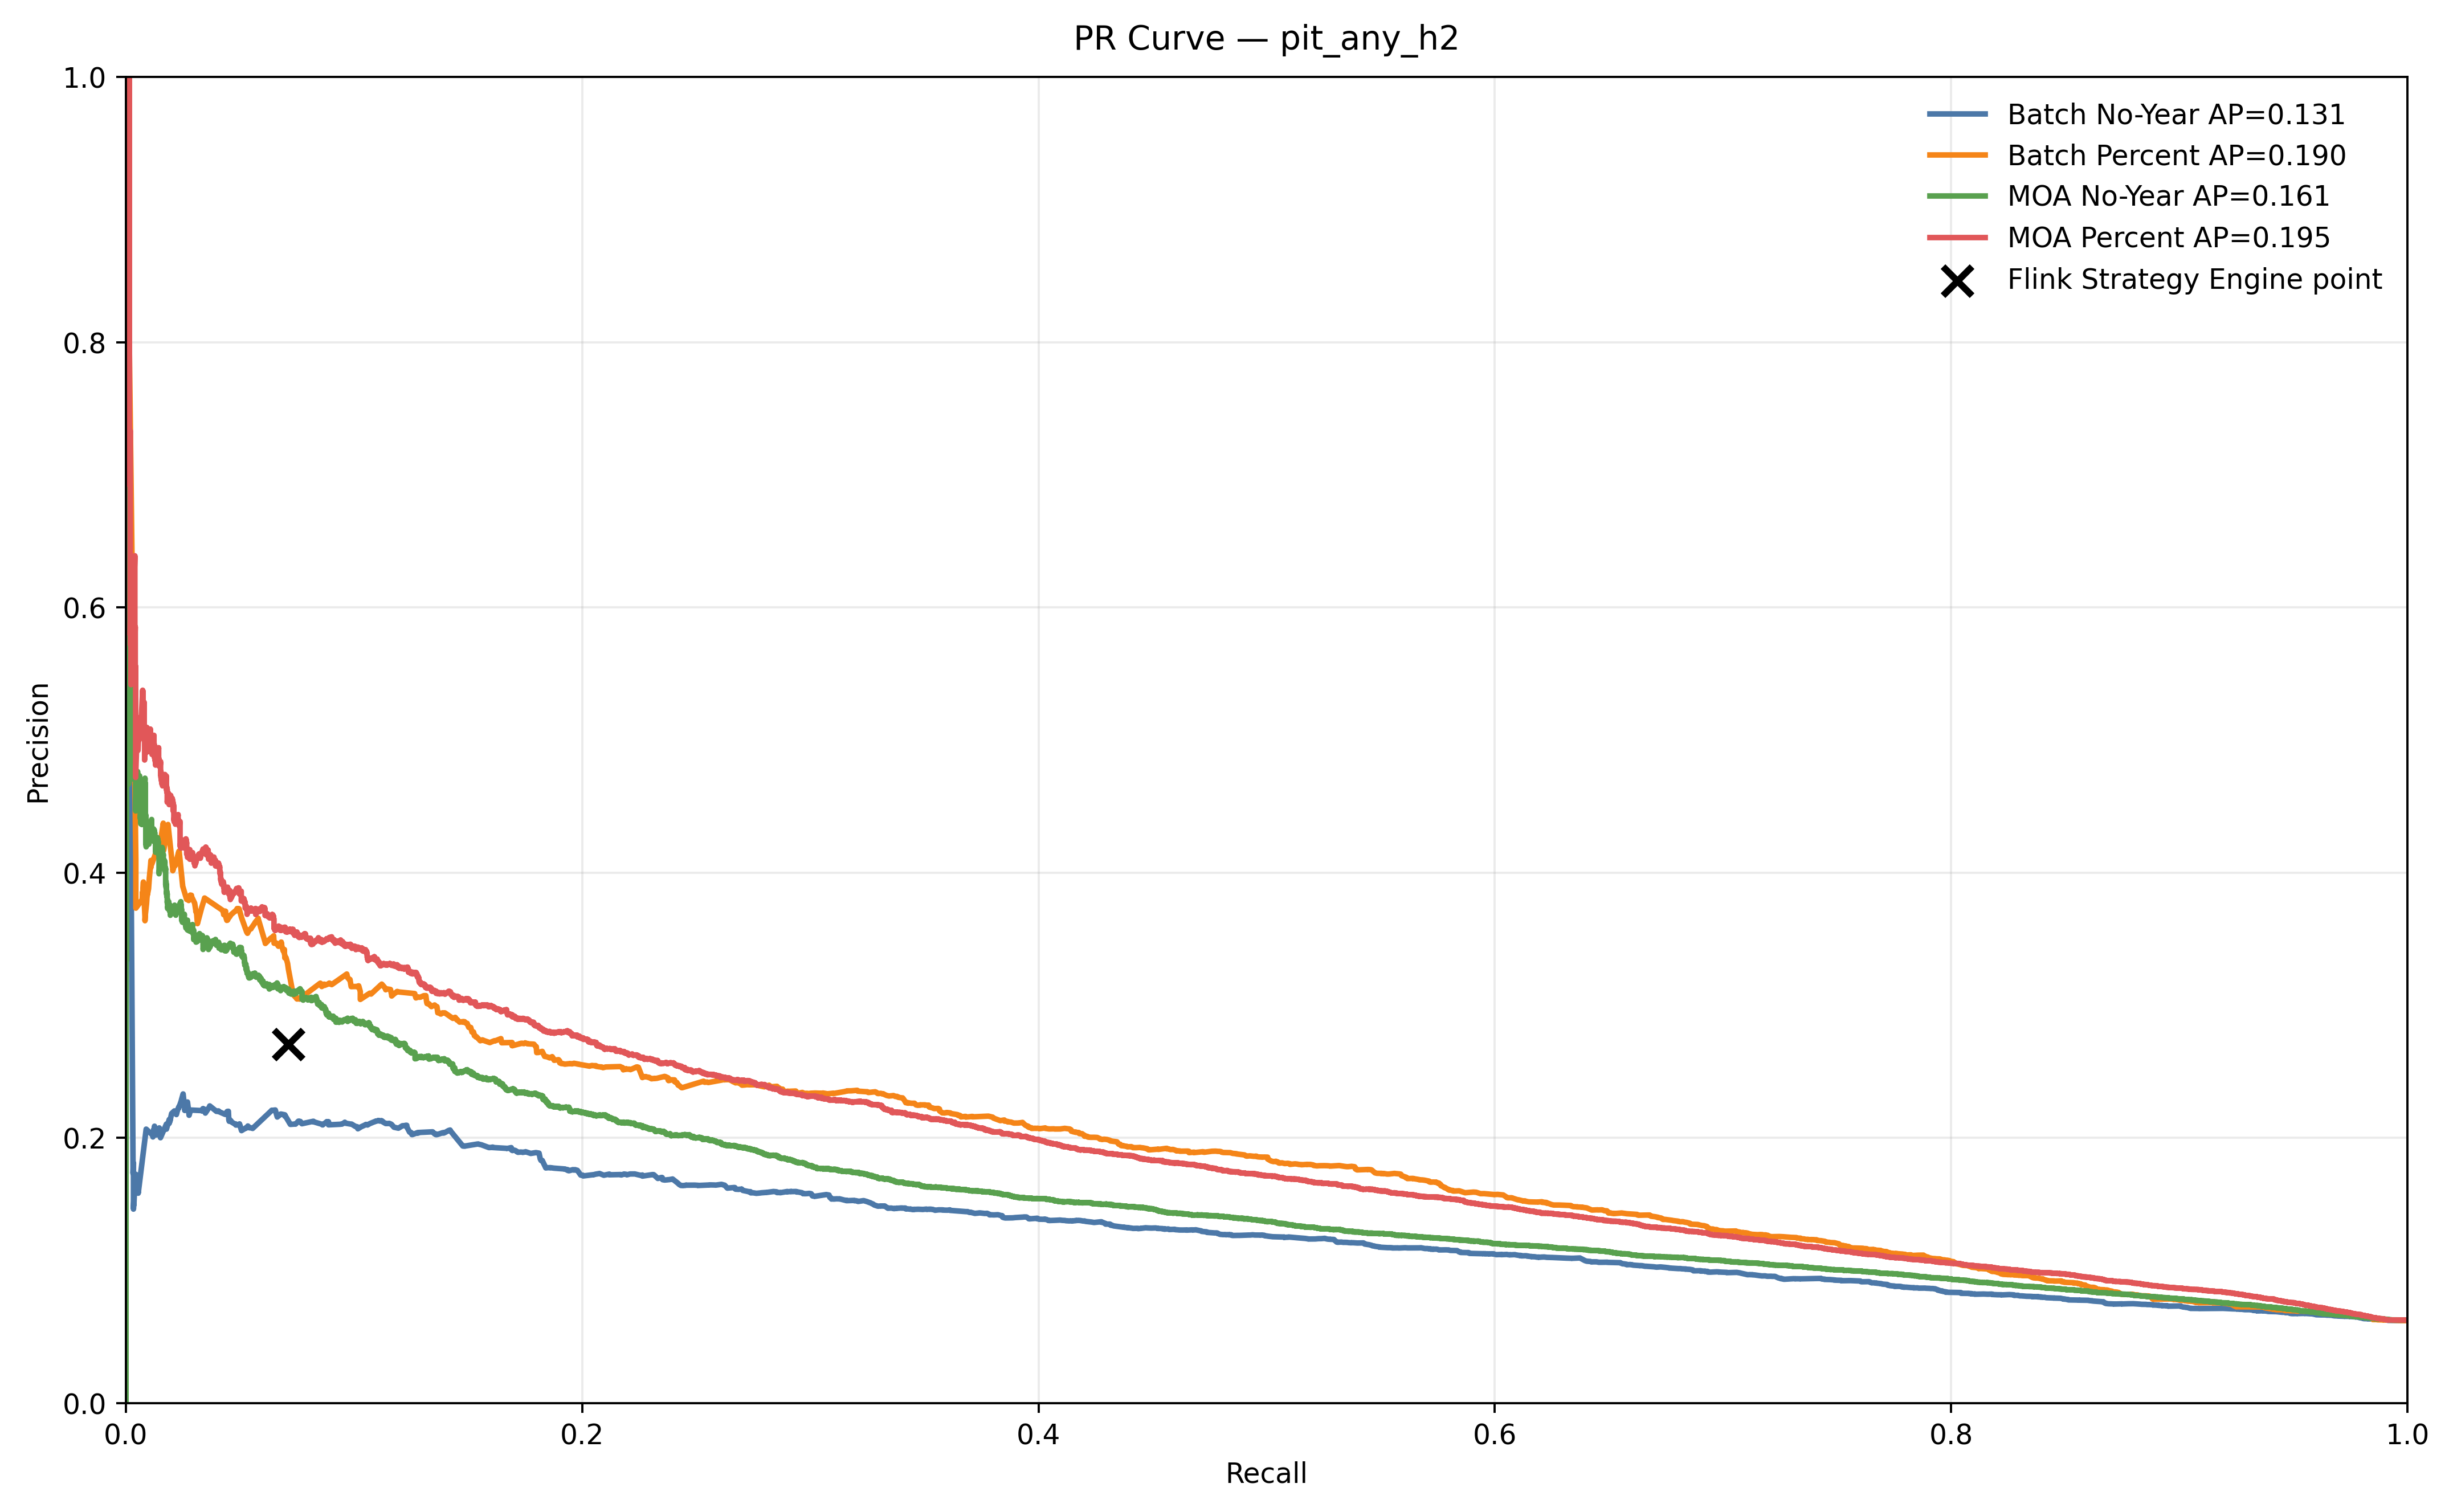
\includegraphics[width=0.85\textwidth]{Images/ch5/pr_curve_pit_any_final.png}
    \caption{Precision--recall curve for \texttt{pit\_any\_h2}.}
    \label{fig:pr_curve_pit_any_final}
\end{figure}

\begin{figure}[htbp]
    \centering
    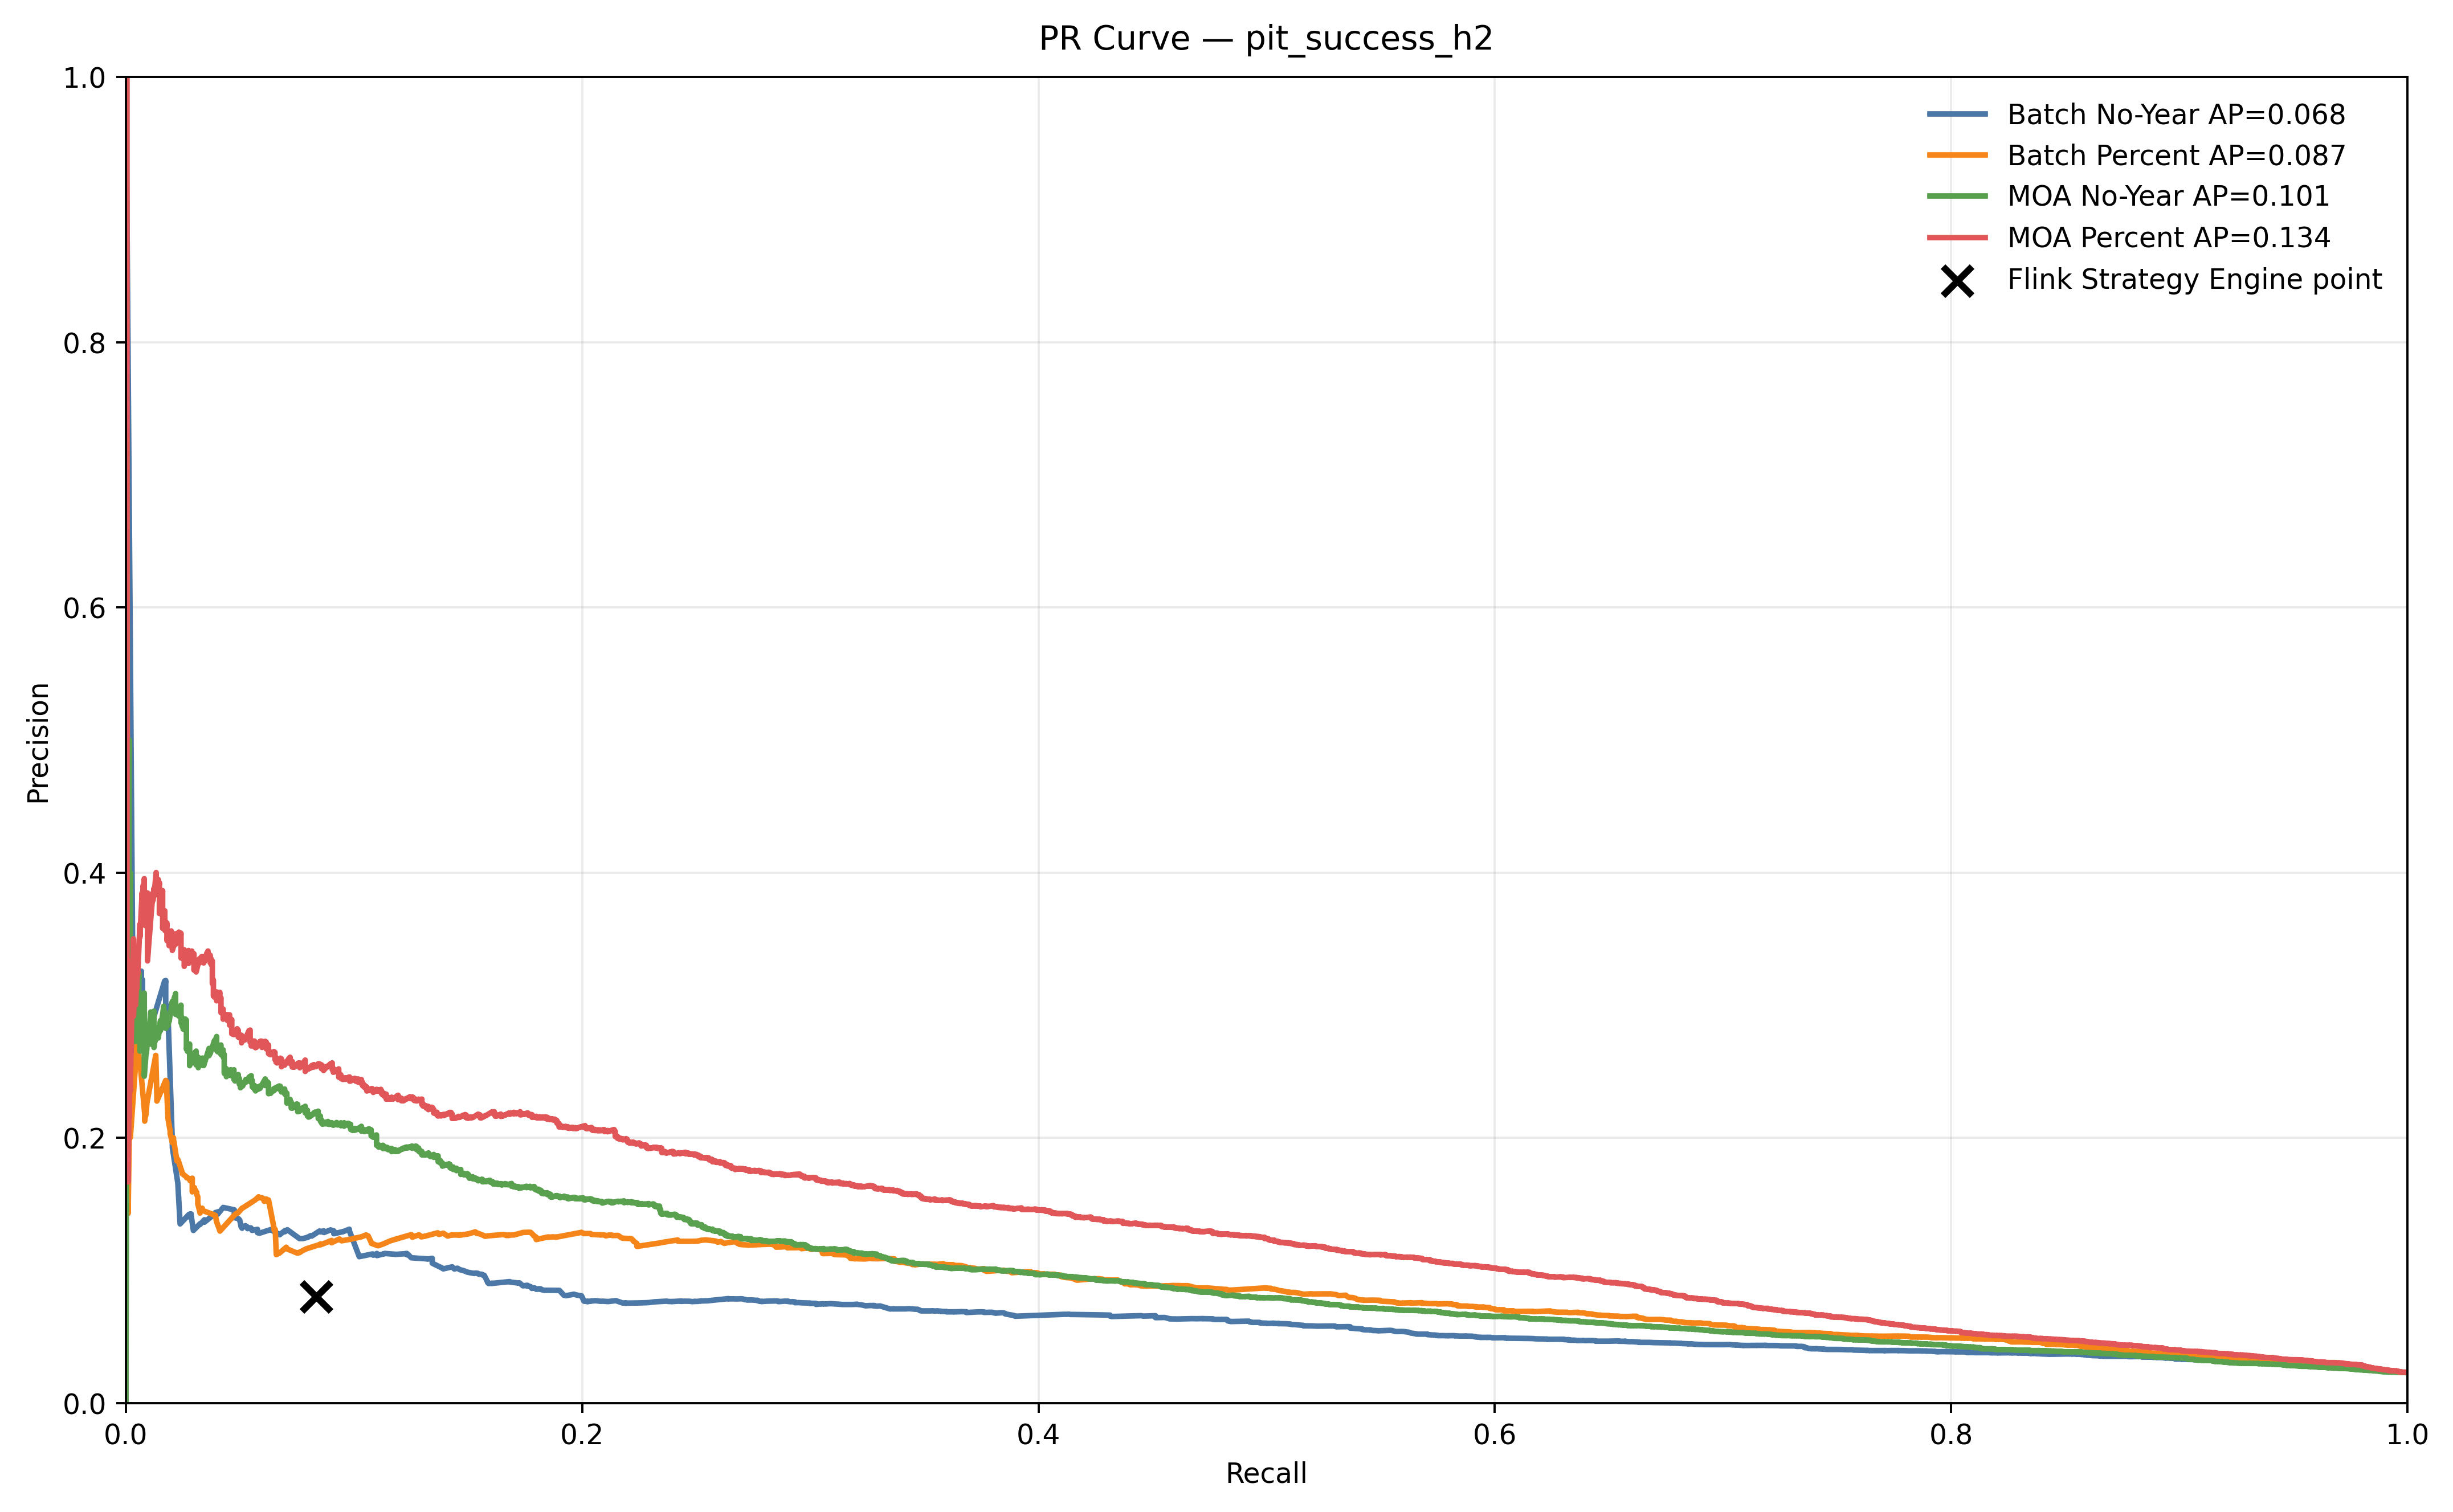
\includegraphics[width=0.85\textwidth]{Images/ch5/pr_curve_pit_success_final.png}
    \caption{Precision--recall curve for \texttt{pit\_success\_h2}.}
    \label{fig:pr_curve_pit_success_final}
\end{figure}

Table~\ref{tab:ap_summary_final} reports Average Precision for the score-based systems. For both targets, MOA Percent obtains the highest AP. 
On \texttt{pit\_any\_h2}, Batch Percent is close to MOA Percent, which is consistent with the strong timing behaviour already observed in the 
selected operating points. On \texttt{pit\_success\_h2}, the AP values are lower overall, confirming that the success task is harder to rank 
as well as harder to classify under a fixed threshold.

\begin{table}[htbp]
    \centering
    \caption{Average Precision for score-based systems. AP is a row-level ranking diagnostic, not operational precision.}
    \label{tab:ap_summary_final}
    \begin{tabular}{lcccc}
        \toprule
        Target                  & Batch No-Year & Batch Percent & MOA No-Year & MOA Percent \\
        \midrule
        \texttt{pit\_any\_h2}     & 0.131         & 0.190         & 0.161       & 0.195 \\
        \texttt{pit\_success\_h2} & 0.068         & 0.087         & 0.101       & 0.134 \\
        \bottomrule
    \end{tabular}
\end{table}

The AP table should be read together with the headline metrics. A model can have a useful ranking curve while still requiring a conservative threshold 
to obtain acceptable operational precision. This is especially visible for \texttt{pit\_success\_h2}, where the best AP belongs to 
MOA Percent, but the selected operating point still has low successful event coverage.

\section{Support-Aware Race-Level Diagnostics}

\subsection{\texttt{pit\_any\_h2}: Kappa and G-Mean per race}

% Slide 53 (Kappa) + Slide 54 (G-Mean).
%
% Goal:
% Show race-level variability under minimum positive support filtering.
%
% Verified support filter and kept races:
% \begin{itemize}
%     \item positives\_min\_filter = 3.
%     \item pit\_any: Flink 92, Batch No-Year 91, Batch Percent 91, MOA No-Year 92, MOA Percent 92.
% \end{itemize}
%
% Artifact anchors:
% \begin{itemize}
%     \item \path{data_lake/reports/phase2b_presentation_figures/final_refresh/race_level_kappa_pit_any.png}
%     \item \path{data_lake/reports/phase2b_presentation_figures/final_refresh/race_level_gmean_pit_any.png}
%     \item \path{data_lake/reports/phase2b_presentation_figures/final_refresh/race_level_support_summary.csv}
% \end{itemize}

\subsection{\texttt{pit\_success\_h2}: Kappa and G-Mean per race}

% Slide 55 (Kappa) + Slide 56 (G-Mean).
%
% Goal:
% Show that strict pit-success race-level diagnostics are much sparser and often near zero.
%
% Verified support filter and kept races:
% \begin{itemize}
%     \item positives\_min\_filter = 3.
%     \item pit\_success: Flink 87, Batch No-Year 86, Batch Percent 86, MOA No-Year 87, MOA Percent 87.
% \end{itemize}
%
% Artifact anchors:
% \begin{itemize}
%     \item \path{data_lake/reports/phase2b_presentation_figures/final_refresh/race_level_kappa_pit_success.png}
%     \item \path{data_lake/reports/phase2b_presentation_figures/final_refresh/race_level_gmean_pit_success.png}
%     \item \path{data_lake/reports/phase2b_presentation_figures/final_refresh/race_level_metric_summary.csv}
% \end{itemize}
%
% Writing caution:
% \begin{itemize}
%     \item treat Kappa/G-Mean as diagnostics (support-sensitive), not headline metrics.
% \end{itemize}


\section{Explainability as Methodology Debugging}
\label{sec:explainability}

\subsection{Explainability role across systems}

% Slide 57.
%
% Goal:
% Explain why explainability is presented as debugging/interpretation support.
%
% Slide-grounded content to keep:
% \begin{itemize}
%     \item Batch XGBoost: direct SHAP / TreeSHAP on trained model.
%     \item MOA Online Learner: surrogate SHAP proxy.
%     \item Flink Strategy Engine: rule logic is interpretable by construction.
% \end{itemize}
%
% Important consistency line:
% \begin{itemize}
%     \item this section supports methodological choices (e.g., No-Year correction), not claims of causal feature effects.
% \end{itemize}

\subsection{\texttt{\_source\_year} shortcut-risk and No-Year correction}

% Slide 58 + Slide 59.
%
% Goal:
% Link explainability findings to protocol corrections already described in Chapter 4.
%
% Slide-grounded claims to keep:
% \begin{itemize}
%     \item \texttt{\_source\_year} appeared as shortcut-risk in Batch explainability.
%     \item this motivated No-Year as the clean neutral baseline.
%     \item Percent profile is engineered, not a fully neutral comparison.
% \end{itemize}
%
% Provenance note (important):
% \begin{itemize}
%     \item Current \texttt{final\_refresh/} package contains the corrected evaluation tables/figures but does not include a dedicated SHAP CSV set.
%     \item If the SHAP comparison figure from Slide 59 is inserted in thesis, add explicit provenance to the exact image-generation artifact used (currently available in local archive history).
% \end{itemize}
%
% TODO: add reproducible explainability artifact path (or regenerate into a tracked thesis-facing location before final submission).


\section{Threats to Validity}

% Map to the closing cautionary points embedded across Slides 50--59.
%
% Threats to include:
% \begin{itemize}
%     \item support sparsity and race-level volatility (especially strict pit\_success).
%     \item threshold-policy dependence for operational behavior.
%     \item comparator-contract dependence (window semantics and unknown handling).
%     \item surrogate explainability limits for online learners.
% \end{itemize}
%
% Suggested anchors:
% \begin{itemize}
%     \item \path{data_lake/reports/phase2b_presentation_figures/final_refresh/race_level_support_summary.csv}
%     \item \path{data_lake/reports/phase2b_presentation_figures/final_refresh/pit_success_threshold_sensitivity_slide.csv}
%     \item \path{data_lake/reports/phase2b_presentation_figures/final_refresh/final_slide_assets_manifest.csv}
% \end{itemize}


% Writing rule for Chapter 5:
% Every numeric claim must be traceable to a file under
% \path{data_lake/reports/phase2b_presentation_figures/final_refresh/}
% or to an explicitly cited upstream source listed in
% \path{data_lake/reports/phase2b_presentation_figures/final_refresh/final_refresh_input_provenance.csv}.

\chapter{Conclusions and Future Work}
\label{ch:conclusions}

\section{Conclusions}

This thesis addressed the problem of evaluating pit decision support systems from historical Formula 1 data under live-like temporal constraints, the implemented system
starts from historical race sessions, converts them into replayable event streams, processes them through a Flink based strategy pipeline, and then compares three decision
paradigms under shared evaluation contracts: the Flink Strategy Engine, Batch XGBoost, and the MOA Online Learner.

A pit recommendation is emitted at a specific driver-lap, while its correctness can only be assessed later,
after the race has evolved and the pit event, if any, has occurred. The evaluation therefore had to connect decision rows, future pit events, and post pit outcome labels
without using future information as model input. This led to the two contracts used throughout the thesis: \texttt{pit\_any\_h2}, for pit timing, and \texttt{pit\_success\_h2},
for successful pit-call prediction.

The final evaluation showed that these two contracts describe different levels of difficulty, where Pit timing can be learned from replayed race context with useful precision
and coverage trade-offs, while Successful pit-call prediction can also be evaluated under a strict operational view, but it remains sparse, threshold sensitive, and harder
to cover reliably. The following findings summarize the main outcomes of the work.

\subsection{Principal Findings}

\begin{enumerate}
    \item \textbf{Aligned contracts are necessary for a fair comparison.}

          The experiments showed that the three systems cannot be compared directly from their native outputs. The Flink Strategy Engine emits rule based labels, Batch
          XGBoost emits out-of-fold scores, and MOA emits vote based scores in prequential order. A meaningful comparison required a shared truth universe, explicit truth
          lenses, leakage filtering, and a clear separation between row-level decisions and event-level coverage. These elements are part of the contribution of the thesis,
          because they define the conditions under which deterministic rules, Batch learning, and online learning can be judged on the same evidence.

    \item \textbf{\texttt{pit\_any\_h2} is the cleaner learnable task.}

          The pit timing contract gave the clearest learning signal. It checks whether an eligible pit stop happens within the evaluation horizon, without asking whether
          that pit is later classified as strategically successful. Under this contract, the learning based systems improved over the deterministic Flink Strategy Engine.
          Batch Percent reached the largest event recall, while MOA gave the strongest precision oriented balance. The task remains imbalanced, but the results indicate
          that race context features such as pace, tyre life, gaps, and race progress contain usable signal for predicting that a pit window is approaching.

    \item \textbf{\texttt{pit\_success\_h2} is stricter and policy-sensitive.}

          The success contract was substantially harder. A positive call is correct only when it matches a future eligible pit and the post pit evaluator classifies that
          pit as successful. This reduces the amount of clean positive evidence and makes the selected operating threshold much more influential. MOA Percent produced the
          cleanest selected successful pit calls, but its successful event coverage remained low. The relaxed threshold analysis confirmed the expected trade-off: coverage
          can be increased, but only by accepting more false positives under the strict operational view.

    \item \textbf{The Flink Strategy Engine remains useful as an interpretable baseline.}

          The rule based system did not dominate the strict precision results, but it provided an interpretable reference point. Its decisions can be followed through explicit
          score terms, gates, and promotion rules. The evaluation also showed why diagnostic matched pit quality must be separated from operational precision. When a Flink call
          matches a known pit, many of those matched pits correspond to successful outcomes. Once no-match calls and failed matched pits are counted as false positives, strict
          precision becomes much lower. This distinction prevents the deterministic baseline from being overstated and keeps the comparison with Batch and MOA fair.

\end{enumerate}

Taken together, these findings answer the two main contract questions of the thesis; pit timing is a learnable decision support task in the implemented replay setting,
successful pit-call prediction can be evaluated under a stricter contract, but the results show a more limited and fragile signal. The strongest conclusion is 
that each paradigm occupies a different position in the trade-off between interpretability, coverage, precision, and temporal evaluation.

\section{Scope and Limitations}

The results should be read within the scope of the implemented pipeline; the first boundary is the use of historical replay, replaying FastF1 sessions through Kafka and
Flink makes the experiments reproducible and gives the system live-like temporal semantics, the same race can be replayed multiple times, the produced artifacts can be
inspected, and the comparison can be regenerated. A live race feed would introduce additional issues, such as data corrections, missing fields, feed latency, and operational
failure modes. The current system is therefore a controlled experimental environment rather than a deployed pit-wall tool usable in production for real world applications.

A second boundary concerns the definition of successful pit outcomes, the \texttt{pit\_success\_h2} target depends on the \texttt{PitStopEvaluator}, which classifies completed
pit cycles from post pit evidence. This gives the thesis a reproducible truth contract, but it does not represent the full utility function of a racing team because a real strategy
decision may also depend on tyre allocation, risk tolerance, team objectives, opponent response, long-term stint plans, or championship context. The evaluator captures part of
the strategic outcome, mainly through gap and rival evolution, but it remains an heuristic approximation.

The strict success contract also creates a support problem, successful pit events are rarer than pit timing events, and some races contain only a small number of clean
positive cases. Race-level Kappa and G-Mean diagnostics therefore become noisy for \texttt{pit\_success\_h2}, even after support filtering. This sparsity limits how strongly
per race behaviour can be interpreted.

Threshold choice is another limitation since Batch XGBoost and MOA produce scores, and the final operational behaviour depends on where the threshold is placed. The selected
thresholds define the headline policies, while the relaxed rows show how quickly the balance between precision and coverage can change. A fixed threshold is useful for
reproducibility, but it cannot represent every possible operational preference.

The MOA branch adds two further boundaries; its positive scores are derived from class votes and are treated as ranking scores, they support
threshold sweeps and precision--recall diagnostics, but they should not be read as direct probabilities of a pit event. The same caution applies to explainability, Batch
XGBoost can be inspected directly through SHAP and TreeSHAP, while the MOA Online Learner does not expose an equally direct attribution path. A surrogate SHAP analysis was
explored, but it was not retained because the surrogate model could not be verified as a faithful explanation of the internal online learner.

Finally, the model comparison is deliberately scoped; the Batch branch uses XGBoost and the online branch uses the selected MOA configuration. This is enough to evaluate the
proposed framework across deterministic, Batch, and online paradigms, but it does not exhaust the space of possible learners. Other Batch models, online learners, calibration
methods, and drift-aware algorithms may produce different trade-offs under the same contracts.

These limitations define what the comparison actually supports: a reproducible evaluation of three decision paradigms on historical
replay data, under explicit contracts and controlled accounting rules. They also indicate where future work should extend the system.

\section{Future Work}

The implemented pipeline provides a foundation for several extensions, the most relevant ones follow directly from the limitations described above.

\subsection{From Historical Replay to Live Ingestion}

The first extension is the transition from replay to live ingestion, the current architecture already separates event sourcing, Kafka streaming, Flink processing,
persisted artifacts, and downstream evaluation. A live version would replace the historical replay source with a real timing or telemetry feed, while keeping the same
stateful processing logic where possible.

This step would test a different part of the system, in replay the input sequence is frozen and can be regenerated while in a live setting, events may arrive late, be
corrected, or be partially unavailable. The system would need stronger monitoring, latency checks, and failure handling, also the evaluation would also have to distinguish
between decisions made with incomplete live data and decisions made after corrected data become available.

\subsection{Richer Truth Models for Successful Pit Outcomes}

The second direction concerns the successful pit truth model. The current \texttt{PitStopEvaluator} provides a deterministic classification of completed pit cycles,
which was necessary for this thesis, a richer evaluator could use longer post pit windows, better rival tracking, tyre compound plans, and more detailed traffic evolution.
It could also include sampled human validation, especially for ambiguous pit cycles where the rule based classification is less clear.

Another possible development is a probabilistic success label, instead of assigning only success, failure, or unknown categories, the evaluator could estimate the
confidence of the outcome; this would help in cases where the gap change is small, the rival context changes after the stop, or safety car and weather conditions
distort the comparison.

\subsection{Event Level and Sequence Aware Learning}

The current learning setup uses driver lap rows, this representation is simple and works well with tabular learners, but part of the evaluation is event level. One future
direction is to train models more directly for event coverage, rather than treating each driver lap row as an independent binary example.

Several formulations are possible, for instance the model could predict time to pit, rank pit opportunities within a short horizon, or optimize event coverage under a false positive
budget. Sequence aware models could also use recent lap history directly, instead of relying only on the engineered state available in the current row. This direction is
especially relevant for \texttt{pit\_success\_h2}, where the signal is sparse and isolated row predictions may not capture the full strategic episode.

\subsection{Adaptive Threshold and Risk Aware Policies}

The threshold frontier showed that the same score model can behave differently depending on the selected operating point, future work could replace fixed thresholds
with adaptive policies. A conservative threshold may be appropriate during stable race phases, while a lower threshold may be useful when a rival has just pitted, when
a safety car appears, or when tyre degradation is rapidly increasing.
Risk-aware policies could expose different operating modes, for instance a monitoring mode could favour coverage and emit early warnings, a recommendation mode could require higher
precision before producing an actionable call. This would make the output more flexible and closer to the way a strategy engineer might use a decision support tool.

\subsection{Broader Online Learning and Calibration Aware Evaluation}

The MOA Online Learner was evaluated through one selected configuration, future work could compare additional online learners, including Hoeffding Trees, Adaptive
Random Forests, and other drift aware ensembles. This would clarify whether the observed MOA behaviour depends on the selected learner or whether the same pattern
appears across different online methods.

\subsection{Faithful Explainability for Online Learners}

The final direction concerns explainability for online models, since the Batch branch has a direct explanation path through tree based attribution, while the MOA branch does not; a
future version could investigate explanation methods designed for streaming learners, or log additional interpretable signals during prequential prediction.
The goal would be to explain online decisions without replacing the learner with a separate surrogate model, possible approaches include local perturbation diagnostics,
model specific explanations when available, or rule summaries extracted from online behaviour. This would make the online branch easier to inspect and more comparable with
the interpretability of the Flink Strategy Engine and Batch XGBoost.

\section{Final Remarks}

The thesis developed a pipeline for comparing pit decision systems from historical race replay to stream processing, learning, and evaluation. The main outcome is a
structured comparison where pit timing showed the clearest learning gains. Successful pit call prediction remained more difficult, mainly
because success is rarer, evaluator dependent, and sensitive to the operating threshold.

The work also showed that evaluation design matters as much as model choice in this setting, a matched pit diagnostic can suggest good conditional behaviour while strict
operational precision remains low. A score can rank rows well while still requiring a conservative threshold. A feature can improve apparent performance while acting as a
shortcut. These effects are part of the pit decision problem and have to be exposed.

The final contribution is therefore both practical and methodological; practically, the system provides an executable path from historical races to comparable decision artifacts,
methodologically, it defines contracts and accounting rules that make deterministic stream rules, Batch learning, and online learning comparable under the same evidence.

%-------------------------------------------------------------------------
%	BIBLIOGRAPHY
%-------------------------------------------------------------------------

\addtocontents{toc}{\vspace{2em}} % Add a gap in the Contents, for aesthetics
\bibliography{Thesis_bibliography} % The references information are stored in the file named "Thesis_bibliography.bib"

%-------------------------------------------------------------------------
%	APPENDICES
%-------------------------------------------------------------------------

\cleardoublepage
\addtocontents{toc}{\vspace{2em}} % Add a gap in the Contents, for aesthetics
\appendix
% \chapter{Appendix A, Additional Experimental Material}

\section{Artifact Families}

This appendix groups non-headline but relevant evidence.

\begin{itemize}
    \item \textbf{Headline figure pack root:}
    \path{data_lake/reports/phase2b_presentation_figures/}
    \item \textbf{Batch Phase 2B artifacts:}
    \path{data_lake/reports/ml_phase2b_dual_contract_2022_2025/}
    \item \textbf{MOA Phase 2B artifacts:}
    \path{data_lake/reports/sml_phase2b_dual_contract_2022_2025/}
\end{itemize}

\section{Suggested Tables to Include in Final Draft}

\begin{itemize}
    \item Full recommended operating-point tables (all lenses, both contracts).
    \item Per-year comparator summaries and per-year frontier outputs.
    \item Pit-success threshold-policy sensitivity tables.
    \item Race-support diagnostics for sparse-metric interpretation.
\end{itemize}

\section{Suggested Figures to Include in Final Draft}

\begin{itemize}
    \item Headline precision/recall/$F_{0.5}$ comparator bars.
    \item Scored vs row\_tp vs truth-events-covered accounting bars.
    \item Batch and MOA threshold frontiers.
    \item PR/AP diagnostic curves.
    \item Seasonal and race-level stability diagnostics (Kappa/G-Mean family).
    \item Explainability pair: Batch direct SHAP and MOA surrogate SHAP.
\end{itemize}

\section{Historical vs Final Evidence Separation}

Legacy ablation/provenance graph families, when retained, should be catalogued separately from final headline evidence.
Use the current final-refresh manifest as authoritative pointer:
\path{data_lake/reports/phase2b_presentation_figures/final_refresh/final_slide_assets_manifest.csv}

Use this rule in the final manuscript:
\begin{itemize}
    \item only corrected final Phase 2B figures in headline chapters,
    \item historical/legacy visuals only as provenance appendix with explicit labeling.
\end{itemize}

\section{Optional Additional Diagnostics}

\begin{itemize}
    \item Detailed overlap audit for Flink Strategy Engine TP vs Batch/MOA TP sets.
    \item Score-distribution diagnostics for missed Flink Strategy Engine TP cases.
    \item Frontier monotonicity and scored-support diagnostics.
\end{itemize}

\paragraph{Writing note.}
Keep Appendix A as a map of ``where evidence lives''; do not duplicate full tables already available as CSV/MD artifacts.

% \chapter{Appendix B, Implementation and Reproducibility Notes}

\section{Minimal Reproducibility Scope}

This appendix lists the minimal file groups required to reproduce the final experimental results (not the presentation figures).

\subsection{Streaming Data Production and Processing}

\begin{itemize}
    \item Replay data extraction: \path{f1-telemetry-producer/src/prepare_race.py}
    \item Kafka replay sender: \path{f1-telemetry-producer/src/stream_race.py}
    \item Flink topology path:
    \path{f1-telemetry-processor/src/main/java/com/polimi/f1/F1StreamingJob.java}
    \item Flink operators under:
    \path{f1-telemetry-processor/src/main/java/com/polimi/f1/operators/}
\end{itemize}

\subsection{Thesis ML/MOA Experimental Pipeline}

\begin{itemize}
    \item Dataset prep: \path{ml_pipeline/prep_data.py}
    \item Batch training entrypoint: \path{ml_pipeline/train_model.py}
    \item Batch training core: \path{ml_pipeline/lib/model_training_cv.py}
    \item Batch evaluation: \path{ml_pipeline/evaluate_batch_dual_contract_run.py}
    \item Shared universe build: \path{ml_pipeline/build_shared_truth_universe.py}
    \item Frontier builder: \path{ml_pipeline/phase2b_threshold_frontier.py}
    \item MOA export: \path{ml_pipeline/export_moa_dataset.py}
    \item MOA classic prequential run: \path{ml_pipeline/run_moa_arf.py}
    \item MOA continuous vote logger: \path{ml_pipeline/run_moa_vote_logger.py}
    \item MOA vote logger Java source:
    \texttt{MoaPrequentialVoteLogger.java} under \path{ml_pipeline/java_src/}
    \item MOA evaluation: \path{ml_pipeline/evaluate_moa_dual_contract_run.py}
    \item MOA orchestration: \path{ml_pipeline/run_sml_phase2b_dual_contract.py}
\end{itemize}

\section{Frozen Protocol Parameters}

\begin{itemize}
    \item Years: 2022 2023 2024 2025
    \item Horizon: $H=2$
    \item Headline truth universe: \texttt{canonical\_sde\_truth}
    \item Headline lens: \texttt{clean\_actionable}
    \item Profiles:
    \begin{itemize}
        \item \texttt{e0\_no\_source\_year}
        \item \texttt{p1\_percent\_conservative\_v1}
    \end{itemize}
\end{itemize}

\section{Command Skeleton (Core Experiment)}

\subsection{1) Build E0 and P1 datasets}

\begin{verbatim}
OUT_E0=<path_to_e0_dataset.parquet>
OUT_P1=<path_to_p1_dataset.parquet>

.venv/bin/python ml_pipeline/prep_data.py \
  --data-lake data_lake \
  --years 2022 2023 2024 2025 \
  --season-tag season \
  --output "$OUT_E0" \
  --feature-profile baseline \
  --track-agnostic-mode off

.venv/bin/python ml_pipeline/prep_data.py \
  --data-lake data_lake \
  --years 2022 2023 2024 2025 \
  --season-tag season \
  --output "$OUT_P1" \
  --feature-profile percent_conservative_v1 \
  --track-agnostic-mode track_percentage_v1
\end{verbatim}

\subsection{2) Batch OOF + evaluation (race-sequential expanding)}

Use \path{ml_pipeline/train_model.py} +
\path{ml_pipeline/evaluate_batch_dual_contract_run.py}
for both profiles across six targets (raw/clean\_actionable/clean\_dry\_strategy $\times$ pit\_any/pit\_success), storing outputs under:
\begin{verbatim}
data_lake/reports/ml_phase2b_dual_contract_2022_2025/
\end{verbatim}

\subsection{3) Canonical truth universe + Batch frontier}

\begin{verbatim}
.venv/bin/python ml_pipeline/build_shared_truth_universe.py ...
.venv/bin/python ml_pipeline/phase2b_threshold_frontier.py ...
\end{verbatim}

Outputs under:
\begin{verbatim}
data_lake/reports/ml_phase2b_dual_contract_2022_2025/
\end{verbatim}

\subsection{4) MOA Phase 2B orchestration}

\begin{verbatim}
TRUTH_UNIVERSE_CSV=<path_to_canonical_sde_truth_universe_csv>

.venv/bin/python ml_pipeline/run_sml_phase2b_dual_contract.py \
  --years 2022 2023 2024 2025 \
  --run-export --run-moa --run-eval \
  --run-matrix --run-frontier --run-prequential \
  --run-native-sensitivity \
  --truth-universe-race-driver-csv "$TRUTH_UNIVERSE_CSV" \
  --truth-universe-events-csvs ... \
  --moa-jar data_lake/tools/moa.jar \
  --jobs auto --resume
\end{verbatim}

Outputs under:
\begin{verbatim}
data_lake/reports/sml_phase2b_dual_contract_2022_2025/
\end{verbatim}

Typical dataset locations used in this thesis run:
\begin{itemize}
    \item \path{data_lake/ml_training_dataset_2022_2025_dual_contract.parquet}
    \item \path{data_lake/ml_training_dataset_2022_2025_dual_contract_p1_percent.parquet}
\end{itemize}

\section{Mandatory Input Artifacts}

\begin{itemize}
    \item Pit-truth eligibility audits (2022, 2023, 2024, 2025) for \texttt{c6\_cfg120\_fixed}.
    \item Prepared pit-events CSV used by evaluators.
    \item MOA JAR file at \path{data_lake/tools/moa.jar}.
\end{itemize}

\section{Validation and Integrity Checks}

Before claiming results, confirm:
\begin{itemize}
    \item recommended operating-point CSVs exist for Batch and MOA,
    \item canonical compact comparison CSVs exist for Batch and MOA,
    \item SML OOF score uniqueness is continuous (not hard-decision-only),
    \item report tables use row-level and event-level metrics consistently.
\end{itemize}

\paragraph{Writing note.}
Keep Appendix B short and executable. Full bash loops can be referenced from
\path{README.md} and script wrappers.



% LIST OF FIGURES
\listoffigures

% LIST OF TABLES
\listoftables

% LIST OF SYMBOLS
\chapter*{List of Symbols}
\renewcommand{\arraystretch}{1.25}
\begin{longtable}{p{0.20\textwidth}p{0.58\textwidth}p{0.14\textwidth}}
    \textbf{Variable}  & \textbf{Description}                                                                                  & \textbf{Unit} \\
    \hline
    \endfirsthead

    \textbf{Variable}  & \textbf{Description}                                                                                  & \textbf{Unit} \\
    \hline
    \endhead

    $k$                & Current lap at which a decision or prediction is emitted                                              & laps          \\

    $H$                & Prediction horizon used to match positive calls with future pit events                                & laps          \\

    $P$                & Current race position of a driver in the drop-zone computation                                        & position      \\

    $j, m$             & Index variables used when walking the position ladder behind a driver                                 & --            \\

    $lapTime$          & Lap time of the current driver-lap observation                                                        & s             \\

    $stintBestLap$     & Best lap time observed in the current stint for the driver                                            & s             \\

    $thresholdPct$     & Dynamic tyre-drop threshold used to compare the current lap with the stint-best lap                   & ratio         \\

    $compoundBase$     & Base tyre-degradation threshold associated with the tyre compound                                     & ratio         \\

    $fuelAdjust$       & Fuel-related adjustment applied to the tyre-drop threshold                                            & ratio         \\

    $hotTrackAdjust$   & Track-temperature adjustment applied to the tyre-drop threshold                                       & ratio         \\

    $thresholdFloor$   & Minimum allowed value for the dynamic tyre-drop threshold                                             & ratio         \\

    $gapToCarAhead_j$  & Gap from car $j$ to the car immediately ahead in the race order                                       & s             \\

    $pitLoss$          & Estimated time loss caused by a pit stop under the current track-status condition                     & s             \\

    $S$                & Total pit desirability score produced by the Flink Strategy Engine                                    & score         \\

    $S_{pace}$         & Score contribution associated with stint-relative pace degradation                                    & score         \\

    $S_{track}$        & Score contribution associated with track status, such as SC or VSC conditions                         & score         \\

    $S_{traffic}$      & Score contribution associated with the expected traffic or clean-air condition after the pit stop     & score         \\

    $P_{strategy}$     & Strategy penalty applied when the inferred next compound cannot cover the remaining laps              & score         \\

    $S_{action}$       & Action urgency score combining tyre-life urgency and rival reaction pressure                          & score         \\

    $S_{timing}$       & Timing-pressure score associated with local decision-window signals                                   & score         \\

    $P_{eor}$          & End-of-race suppression term used to reduce late unnecessary calls                                    & score         \\

    $B_{competitive}$  & Competitive pressure bonus derived from gaps and recent rival pit activity                            & score         \\

    $P_{uncertainty}$  & Penalty associated with missing or low-confidence race-context signals                                & score         \\

    $g$                & Estimated emergence gap after applying pit loss in the drop-zone computation                          & s             \\

    $deficit$          & Fractional deficit between remaining laps and the estimated maximum stint length of the next compound & ratio         \\

    $lapsRemaining$    & Number of laps remaining in the race at the current observation                                       & laps          \\

    $maxStint_{next}$  & Estimated maximum stint length for the inferred next tyre compound                                    & laps          \\

    $tyreRatio$        & Tyre-life ratio used to compute action urgency                                                        & ratio         \\

    $raceProgress$     & Fraction of the scheduled race already completed                                                      & ratio         \\

    $signalConfidence$ & Confidence score derived from the availability and quality of race-context signals                    & ratio         \\

    $\Delta_{gap}\%$   & Normalized change in gap before and after a pit stop                                                  & \%            \\

    $preGap$           & Gap to the relevant rival before the pit cycle                                                        & s             \\

    $postGap$          & Gap to the relevant rival after the pit cycle                                                         & s             \\

    $baselineLapTime$  & Reference lap time used to normalize the post-pit gap change                                          & s             \\

    $TP$               & True positives: positive calls matched to the required target condition                               & count         \\

    $FP$               & False positives: positive calls that do not satisfy the target condition                              & count         \\

    $FN$               & False negatives: target events or rows not covered by a positive call                                 & count         \\

    $F_{0.5}$          & Precision-weighted F-score used to summarize selected operating points                                & --            \\

    $AP$               & Average Precision, used as a row-level ranking diagnostic                                             & --            \\

    $\kappa$           & Cohen's Kappa, used as a race-level agreement diagnostic                                              & --            \\

    $G$-Mean           & Geometric mean of sensitivity and specificity, used as an imbalance diagnostic                        & --            \\
\end{longtable}


% ACKNOWLEDGEMENTS
\chapter*{Acknowledgements}
% add acknowledgements here

\begingroup
\renewcommand{\thesection}{\arabic{section}}
\setcounter{section}{0}

\section{English}

My academic journey would've been impossible without the support of many people, first I would like to thank my supervisor, Prof. Emanuele Della Valle,
for his invaluable guidance and support throughout this thesis, for giving me freedom and trusting me to work on a thesis topic that I am passionate about.

Thanks to my girlfriend Giulia, for her love and encouragement, for being my rock during the challenging moments of this journey, and for always believing in me; believe in
yourself as much as you believe in me and you will achieve anything you set your mind to, because you are truly amazing. I am grateful for your presence in my life and for the
joy you bring to every day, I love you.

Thanks to my mum for her unconditional love and support, for always being there for me, and for teaching me the value of life and perseverance; words cannot express
my gratitude enough.

Thanks to my dad, even if I wasn't lucky enough to get to know you, I can feel your passion and stubbornness in my veins which has been fuel for my ambitions and dreams,
I hope I made you proud, a lot more has to come.

Thanks to my uncle Pepe for his support through my journey, as a fellow Politecnico student you knew how hard it can be sometimes, and your help and advice especially
through my first years were immense.

Thanks to my grandma Carolina and to my grandpa Gigi, for their love and continuous support, I wish I could show grandpa Gigi how much I have achieved and how much I am still
going to achieve, I know you are looking at me from above and cheering for me, thank you.

Thanks to the Tedesi family, for being a second family to me, for their love and support, and for always making me feel welcome and at home, I am grateful to have you in my life.

Thanks to all my family, we are too many to mention but I love you all and I am grateful for having you in my life, I couldn't have been more lucky.

Thanks to all my friends, for the ones at home and the ones I made along my academic journey, for the fun times and the support and strength you all gave me directly
or indirectly, I am glad to have you in my life and I hope we will keep sharing great moments together for many years to come.

Here at Section~\ref{sec:link} of the acknowledgements I want to share a link, it is a video of Ayrton Senna's speech on life and achievements, it is a great source of motivation and inspiration
for me, I hope it can be for someone else as well.

Thanks to everyone from the bottom of my heart, this thesis is also yours.


\section{Italian}

Il mio percorso accademico sarebbe stato impossibile senza il supporto di tante persone, per prima cosa vorrei ringraziare il mio relatore, il Prof. Emanuele Della Valle,
per la sua preziosa guida e il suo supporto durante questa tesi, per avermi lasciato libertà e per essersi fidato di me nel lavorare su un argomento che mi appassiona.

Grazie alla mia ragazza Giulia, per il suo amore e il suo incoraggiamento, per essere stata la mia roccia nei momenti più difficili di questo percorso, e per aver sempre creduto in me; 
credi in te stessa tanto quanto credi in me e riuscirai a raggiungere qualsiasi cosa tu voglia, perché sei davvero una persona incredibile. Sono grato di averti nella mia vita e per la
gioia che porti in ogni giorno, ti amo.

Grazie a mia mamma per il suo amore e il suo supporto incondizionati, per esserci sempre stata per me, e per avermi insegnato il valore della vita e della perseveranza; le parole 
non bastano per esprimere tutta la mia gratitudine.

Grazie a mio papà, anche se non ho avuto la fortuna di conoscerti, sento la tua passione e la tua testardaggine scorrere nelle mie vene e alimentare le mie ambizioni e i miei sogni,
spero di averti reso orgoglioso, ma questo è solo l'inizio.

Grazie a mio zio Pepe per il suo supporto durante il mio percorso, da ex studente del Politecnico sapevi quanto potesse essere difficile a volte, e il tuo aiuto e i tuoi consigli 
soprattutto durante i miei primi anni sono stati immensi.

Grazie a mia nonna Carolina e a mio nonno Gigi, per il loro amore e il loro supporto costante, vorrei poter mostrare a nonno Gigi quanta strada ho fatto e quanta ancora
ne voglio fare, so che mi stai guardando da lassù e che fai il tifo per me, grazie.

Grazie alla famiglia Tedesi, per essere stata una seconda famiglia per me, per il loro amore e supporto, e per avermi sempre fatto sentire accolto e a casa, sono grato di avervi nella 
mia vita.

Grazie a tutta la mia famiglia, siamo troppi per nominarvi tutti ma vi voglio bene e sono grato di avervi nella mia vita, non avrei potuto essere più fortunato.

Grazie a tutti i miei amici, sia quelli di casa sia quelli che ho incontrato durante il mio percorso accademico, per i momenti belli e divertenti e per il supporto e la forza che mi 
avete dato direttamente o indirettamente, sono felice di avervi nella mia vita e spero che continueremo a condividere bei momenti insieme per molti anni ancora.

Qui nella Sezione~\ref{sec:link} dei ringraziamenti voglio condividere un link, è un video del discorso di Ayrton Senna sulla vita e sui traguardi, per me è una grande fonte di motivazione e ispirazione
e spero possa esserlo anche per qualcun altro.

Grazie a tutti dal profondo del cuore, questa tesi è anche vostra.

\section{Link}
\label{sec:link}
\begin{center}
    \qrcode[height=2.5cm]{https://youtu.be/nyNwoVRikoc}

    \vspace{1cm}
    \small
    \href{https://youtu.be/nyNwoVRikoc}{Ayrton Senna's speech on life and achievements}

\end{center}

\endgroup


\cleardoublepage

\end{document}
